%=============================
%        Introduction
%=============================
\section{\todo{Introduction}}

KEK, or the High Energy Accelerator Research Organization (Kō Enerugī Kasokuki Kenkyū Kikō), is a
Japanese institution operating the country's largest particle physics laboratory, located in
Tsukuba. KEK provides particle accelerators and essential infrastructure for a wide range of
research fields, including high-energy physics, material science, structural biology, and radiation
science. One of its most notable facilities is SuperKEKB, the world's most advanced
electron-positron collider. SuperKEKB is designed to reach an instantaneous luminosity of up to $80
\times 10^{34} \, \text{cm}^{-2}\text{s}^{-1}$ and has recently completed its commissioning phase.
It accelerates a 7 GeV electron beam in the High-Energy Ring (HER) and a 4 GeV positron beam in the
Low-Energy Ring (LER), which collide at a single interaction point where the Belle II experiment is
conducted. SuperKEKB currently holds the world record for instantaneous luminosity at $4.71 \times
10^{34} \, \text{cm}^{-2}\text{s}^{-1}$~\cite{zhou_luminosity_2023}, surpassing the previous record
set by the LHC.  With a circumference of approximately 3 km, it is the largest lepton collider in
operation.  Similar to CERN, KEK is a large complex housing multiple accelerators and facilities, as
shown in the schematic in \cref{fig:kek:layout_superkekb}.

\begin{figure}[!htb]
    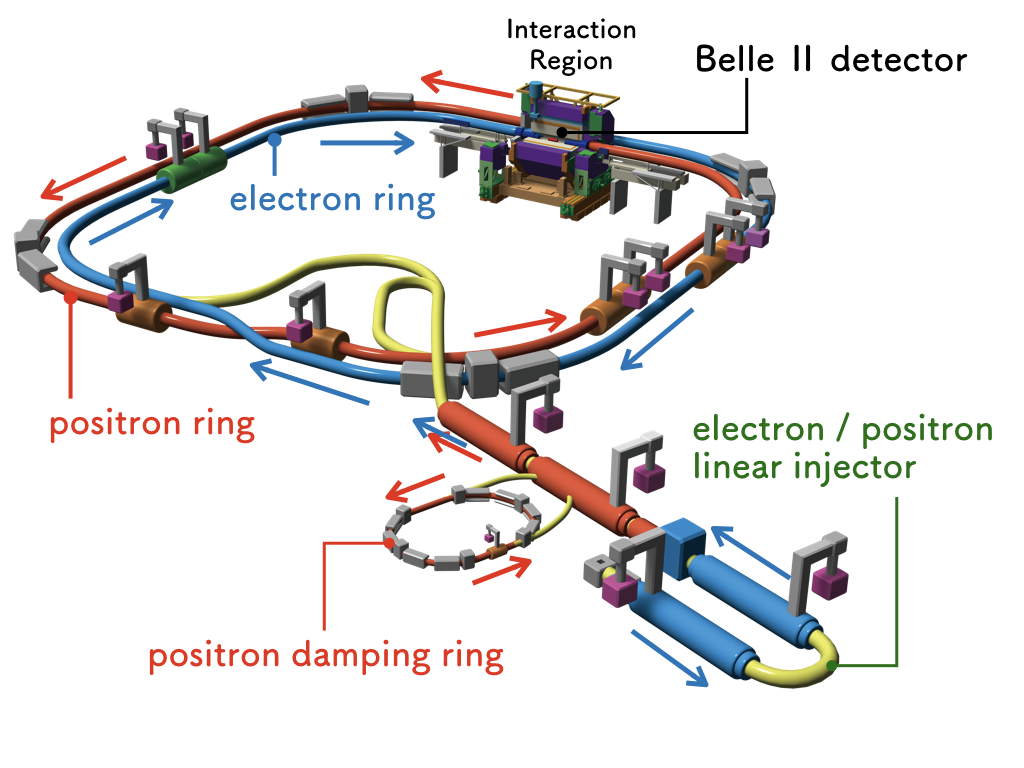
\includegraphics[width=0.8\textwidth]{./images/kek/layout_kekb.jpg}
    \caption{Schematic drawing of the accelerator complex at KEK~\cite{noauthor_operation_2024}.}
    \label{fig:kek:layout_superkekb}
\end{figure}

KEK is currently maintaining collaborations with several organizations, including CERN, to
facilitate research on various topics of interest. SuperKEKB is especially relevant to FCC-ee as it
can act as a prototype for testing innovative manufacturing, measurement, and analysis techniques,
whether in mechanical prototyping, elements alignment, or beam dynamics. During my secondment in
Japan, the optics measurement techniques utilized at CERN for the LHC, specifically turn-by-turn
acquisitions, were tested on the two rings of SuperKEKB. Previous studies have been performed and
are here extended~\cite{keintzel_jacqueline_beam_2022,keintzel_superkekb_2021,keintzel_impact_2021}.



%=============================
%    Measurement Techniques
%=============================
\section{\todo{Measurement Techniques}}

In SuperKEKB, the beam optics are measured using either LOCO (Linear Optics from Closed Orbit) or
turn-by-turn measurements. As fast optics measurements can be achieved with the TbT method, a measurement
campaign has being carried out to improve the measurement quality. This includes investigating
various beam excitation techniques and settings.
The necessary pre-processing steps for optics measurements have been detailed
in~\cite{keintzel_jacqueline_beam_2022}, and are not covered here.


%------------------------------
%    Closed orbit distortion
%------------------------------
\subsection{\todo{Closed Orbit Distortion}}

Optics measurements using the COD method \cite{harrison_global_1987,chung_measurement_1993} are well
established and routinely performed at SuperKEKB. In COD measurements, the beam is excited using six
corrector magnets, and the centroid orbit is recorded by 466 BPMs for the HER and 444 BPMs for the
LER, respectively. The measured orbits, averaged over several turns, are stored in a matrix that
contains a large number of elements. The optics of both transverse planes are then reconstructed
using analytical formulas. Since the correctors must be powered one at a time, the COD method is
relatively time-consuming. 

Another limitation at SuperKEKB is that the feed-down from sextupoles on off-axis particles is 
currently not taken into account, which introduces an error that limits the amplitude of orbit
distortion.  Additionally, since the average particle orbit is observed, the BPM readings are highly
dependent on precise calibration.  One significant advantage of COD measurements at SuperKEKB is
that approximately 6.5 times more BPMs can be used compared to the TbT data.


%------------------------------
%        Turn-by-Turn
%------------------------------
\subsection{\todo{Turn-by-Turn}}

In SuperKEKB, 68 and 70 BPMs in the HER and LER rings are capable of recording turn-by-turn (TbT)
orbit data, typically capturing several thousand turns in both transverse planes. TbT measurements
are usually performed with a single bunch, with currents ranging from 0.2 mA to 1.5 mA. The beam can
be excited using three different methods.

First, an Injection Kicker (IK) delivers a single horizontal kick, causing the beam motion to damp
due to synchrotron radiation. The damping times for the positron and electron rings are 46 ms and 53
ms, corresponding to 4600 and 5300 turns, respectively~\cite{keintzel_jacqueline_beam_2022}.
However, the IK only provides horizontal kicks, limiting the precision of vertical optics
measurements.

In contrast, the Phase-Locked Loop (PLL) method allows continuous excitation of the beam and can
drive both horizontal and vertical planes. The PLL tracks the natural tune of the beam and drives it
at the corresponding frequency. A key advantage of the PLL system is that it can excite both planes
simultaneously, enabling measurements of transverse coupling and other resonance-driving terms
(RDTs). The PLL is currently the only method capable of performing vertical TbT measurements,
although data acquisition must be started manually, and a minimum bunch current of 0.5 mA is
required. This method was not used for the data discussed in this thesis.

The third method is not strictly an excitation. To induce oscillations in the vertical plane, the 
beam can be injected with an orbit offset. This vertical offset causes the beam to oscillate as if 
it had received a single kick. The oscillations then damp, and a new beam must be injected to repeat 
the measurement. This method has been successfully used for the first time to measure vertical
optics using turn-by-turn data.

Once the TbT data is recorded, the standard analysis procedures outlined in
\cref{section:opticcs_meas} are applied. Specifically, the frequency spectrum is calculated before
reconstructing the optics. The model used for this analysis is generated with the SAD (Strategic
Accelerator Design) software \cite{noauthor_sad_nodate}.


%------------------------------
%            GUI
%------------------------------
\subsection{\todo{OMC3 Graphical User Interface}}

The graphical user interface (GUI) used for optics analysis on the LHC, based on OMC3
\cite{omc-team_omc3_2021}, has been updated to support the HER and LER rings of SuperKEKB. This tool
is essential for the rapid and efficient cleaning of bad kicks, BPMs, and for detecting resonance
lines. Utilizing the latest version of the GUI provides access to recent bug fixes and improvements,
enhancing usability and functionality. A typical use case is illustrated in
\cref{fig:kek:gui_bad_bpms}, where BPMs that provide erroneous data across multiple measurements can
be easily identified.

\begin{figure}
    \centering
    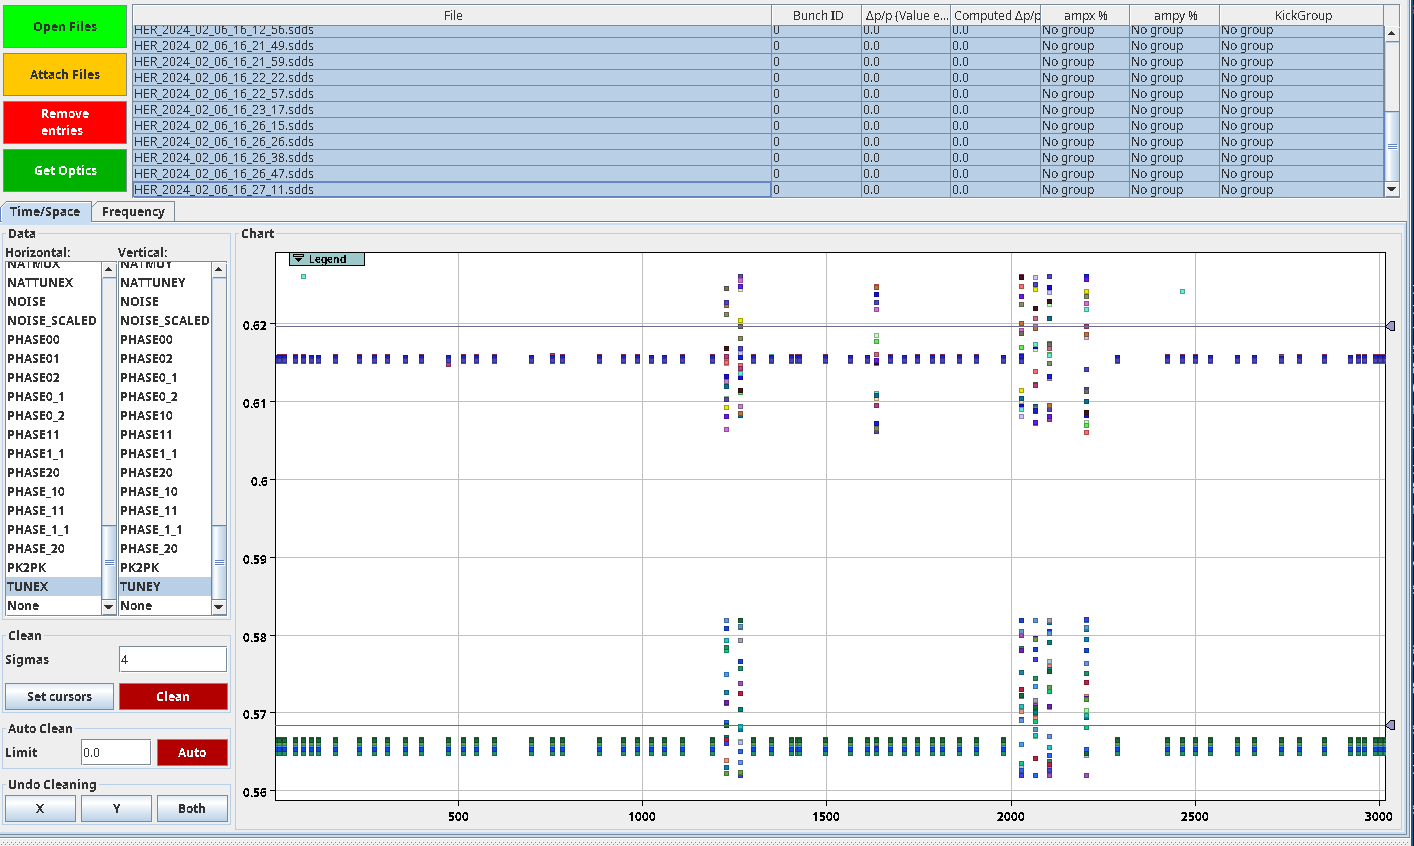
\includegraphics[width=0.9\textwidth]{./images/kek/GUIbadbpm.png}
    \caption{The identification of bad BPMs across measurements is easily done with the GUI.}
    \label{fig:kek:gui_bad_bpms}
\end{figure}



%=============================
%     Optics Observations
%=============================
\section{\todo{Optics Observations}}

All the measurements presented in this section have been performed in February 2024, during the
commissioning phase of SuperKEKB.

%-----------------------------
%        Turn-by-Turn
%-----------------------------
\subsection{\todo{Beta-Beating}}

Several configurations of the machine were measured using turn-by-turn acquisitions, as detailed in
\cref{tab:superkekb:configurations}. The configurations with $\beta_y^* = 48.6$ in LER and
$\beta_y^* = 81$ in HER are referred to as \textit{detuned}. Multiple kicks were performed for each
configuration to increase measurement precision. Although additional measurements were taken,
insufficient kick amplitude in some cases made it challenging to extract reliable linear optics
data and are thus here not included. Specifically, vertical measurements are challenging to perform
as oscillation amplitudes are often low due to the limited achievable offset.
A typical turn-by-turn signal is depicted in \cref{fig:kek:tbt_signal}.
Overall, both the \textit{detuned} and \text{8mm squeezed} optics have been reliably measured for
both rings. However, vertical measurements for the squeezed optics are still challenging to measure 
in LER.

\begin{table}
    \centering
    \begin{tabular}{llrrrrr}
    \hline
    Ring & Day & $\beta_x^*$ [mm] & $\beta_y^*$ [mm] & $Q_x$ & $Q_y$ & Kicks\\
    \hline
    LER        & 06 & 384 &\textbf{48.6} & 44.556 & 46.635 & H \& V \\
               & 09 & 384 &\textbf{48.6} & 44.553 & 46.621 & H  \\
               \hdashline
               & 20 & 200 & \textbf{8}   & 44.527 & 46.604 & H \\
               & 22 & 200 & \textbf{8}   & 44.535 & 46.590 & H \\
               &&&&&& \\
    HER        & 06 & 400 & \textbf{81}  & 45.572 & 43.616 & H \& V\\
               \hdashline
               & 20 & 200 & \textbf{8} & 45.530 & 43.595 & H \\
               & 22 & 200 & \textbf{8} & 45.535 & 43.596 & V \\
               & 26 & 200 & \textbf{8} & 45.535 & 43.596 & V \\
    \bottomrule
    \end{tabular}
  \caption{Configurations of the HER and LER rings for measurements performed via turn-by-turn
  acquisition.}
  \label{tab:superkekb:configurations}
\end{table}


\begin{figure}[!htb]
    \centering
    \begin{subfigure}[b]{0.47\textwidth}
        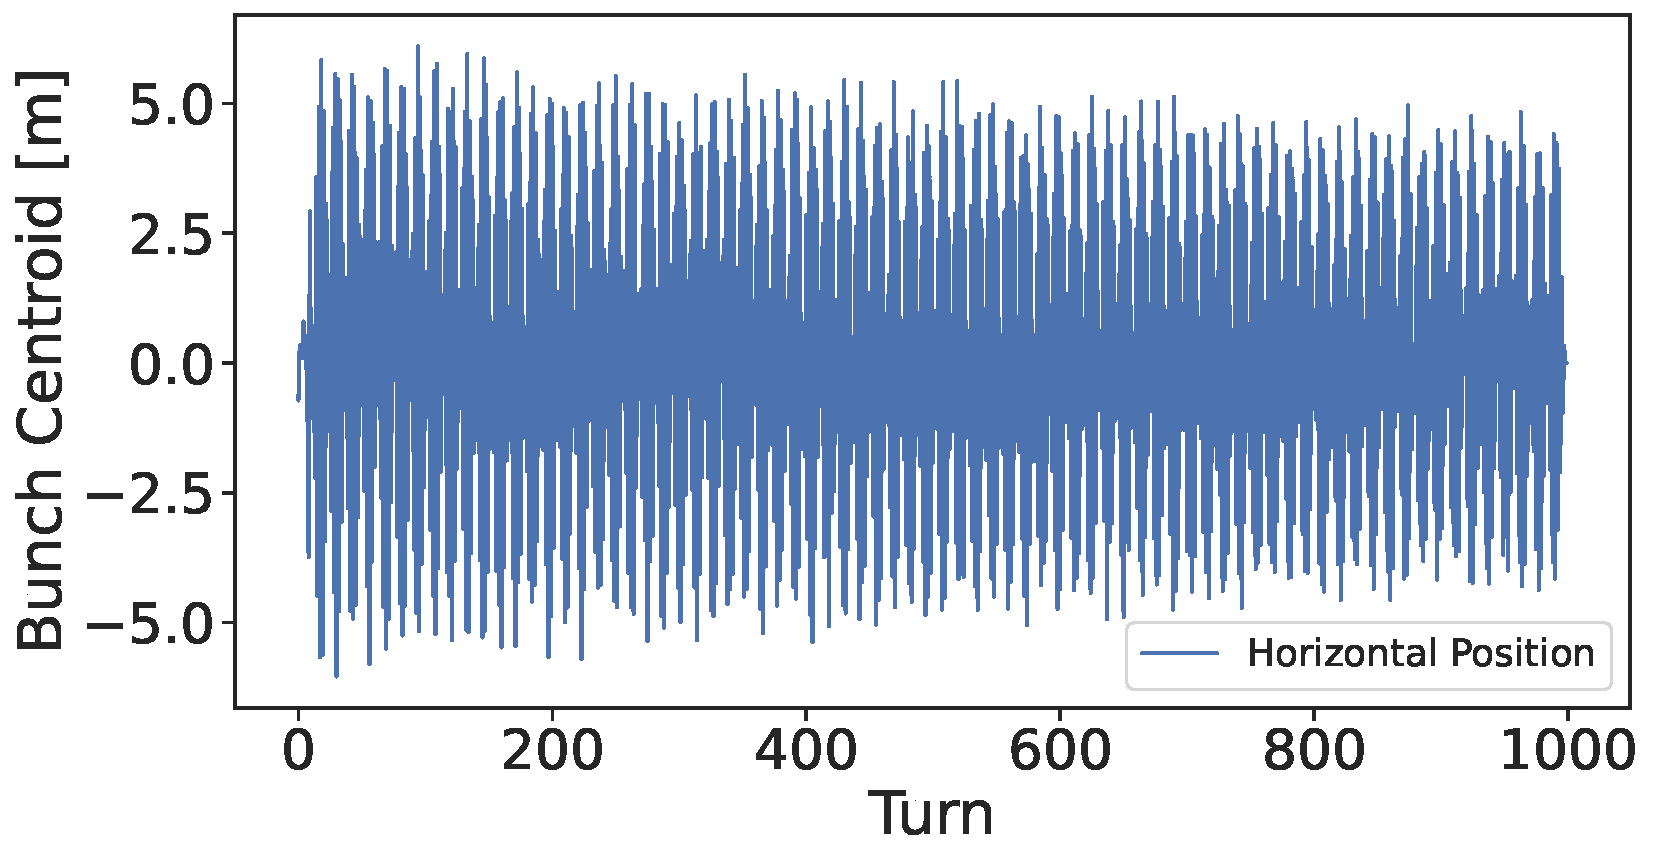
\includegraphics[width=\linewidth]{images/kek/horizontal_tbt_ler.pdf}
        \caption{Horizontal plane, oscillations are created by the Injection Kicker.}
    \end{subfigure}
    \hfill
    \begin{subfigure}[b]{0.48\textwidth}
        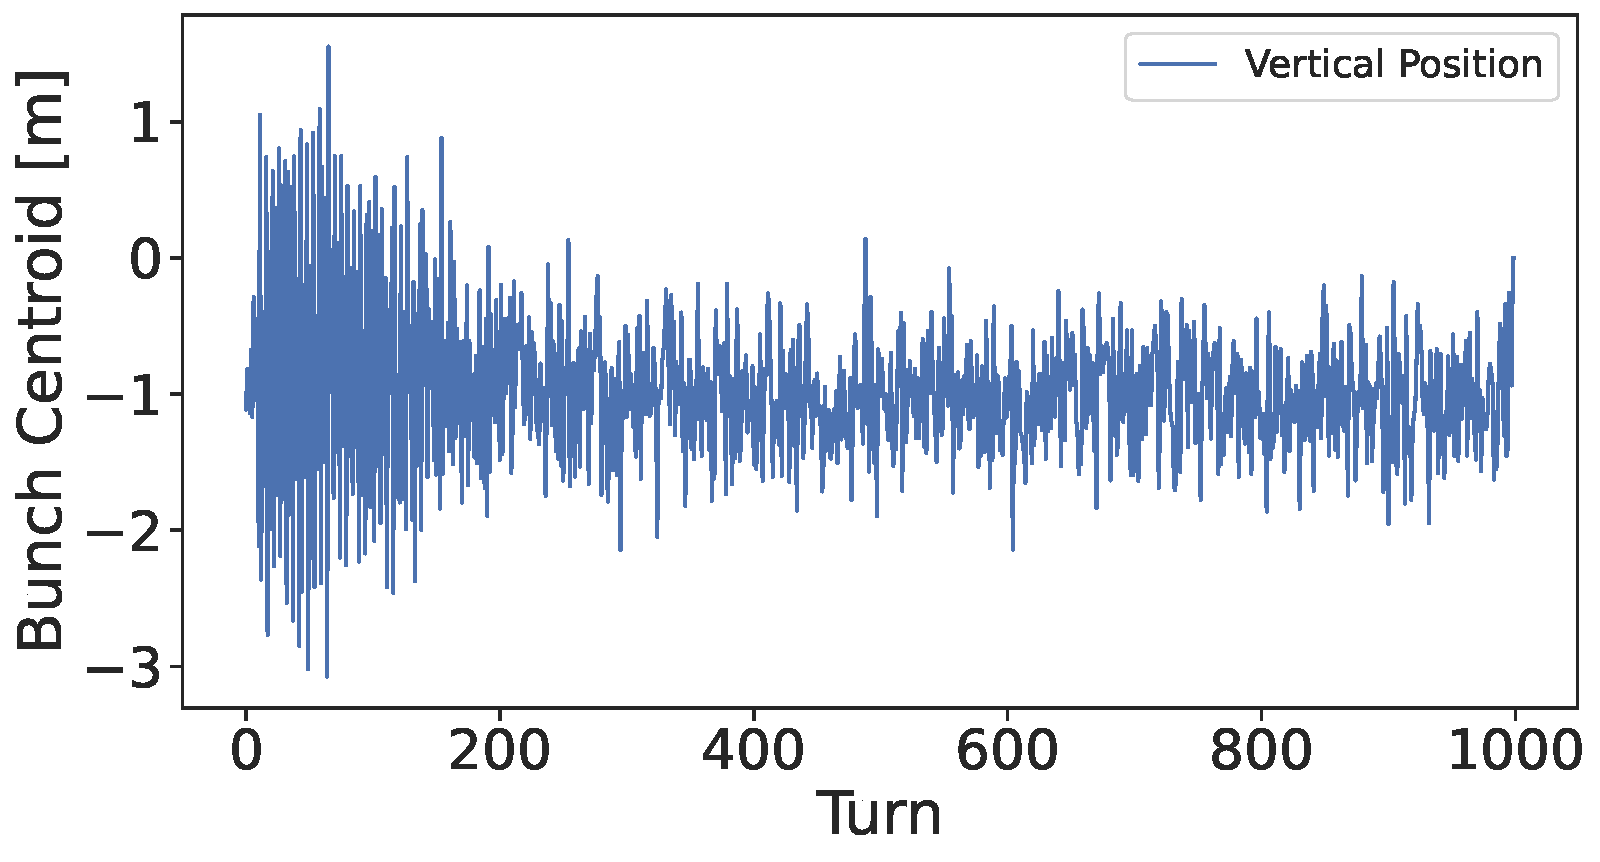
\includegraphics[width=\linewidth]{images/kek/vertical_tbt_ler.pdf}
        \caption{Vertical plane, oscillations are created via an injection offset.}
    \end{subfigure}
    \caption{Typical horizontal and vertical recorded turn-by-turn signal.}
    \label{fig:kek:tbt_signal}
\end{figure}



%-----------------------------
%            LER 
\FloatBarrier
\subsubsection{\todo{LER $\beta-beating$}}

\begin{figure}[!htb]
    \centering
    \begin{subfigure}[b]{0.48\textwidth}
        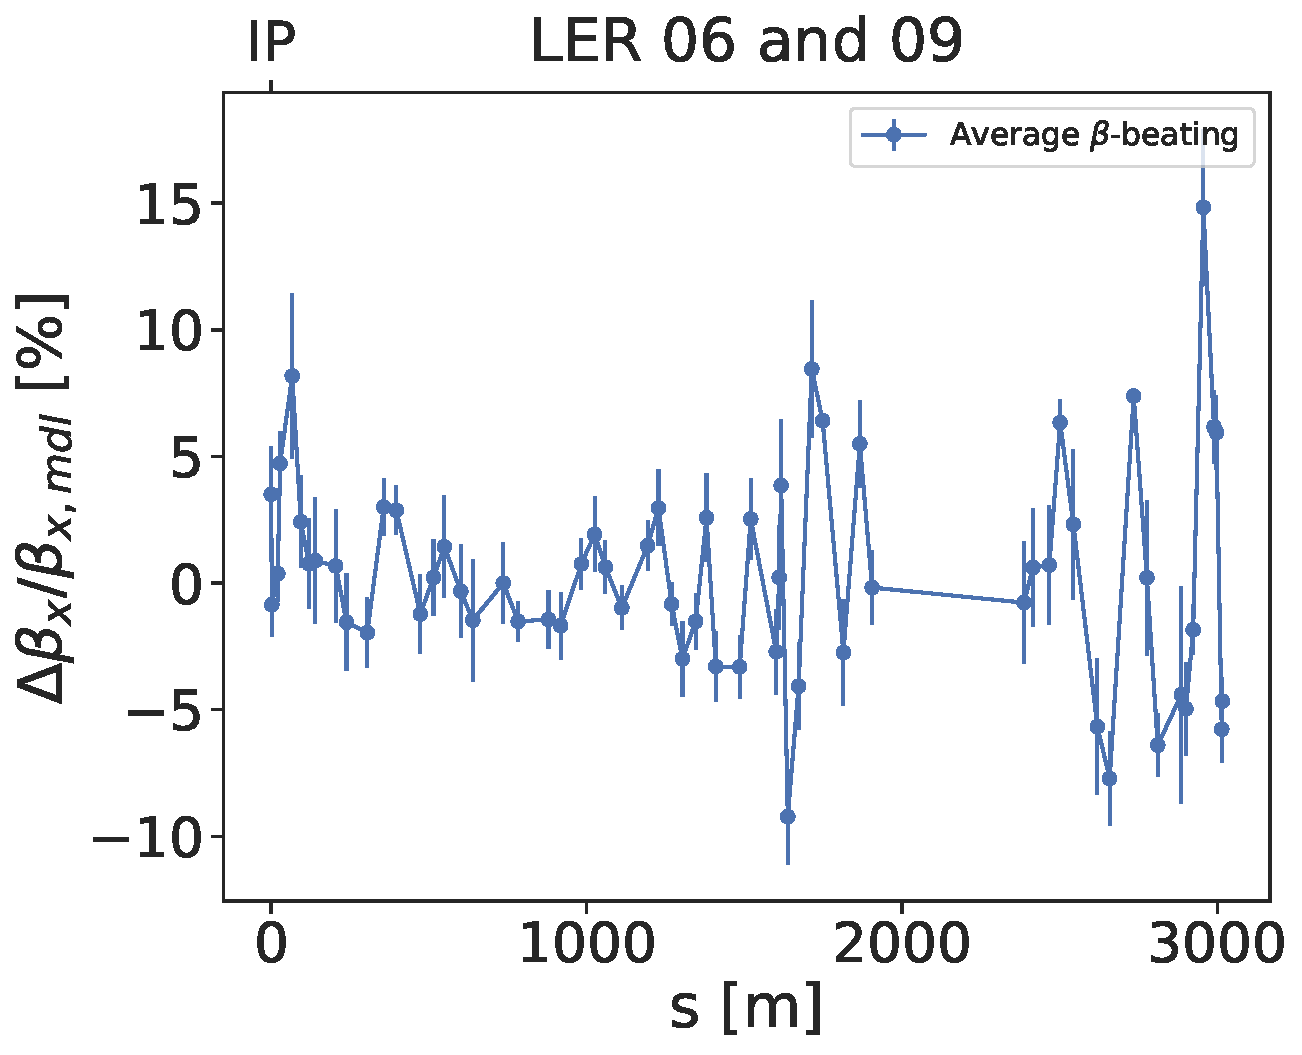
\includegraphics[width=\linewidth]{images/kek/ler_06_09_bet_x.pdf}
        \caption{Horizontal beta-beating, RMS is $\approx 4\%$.}
    \end{subfigure}
    \hfill
    \begin{subfigure}[b]{0.48\textwidth}
        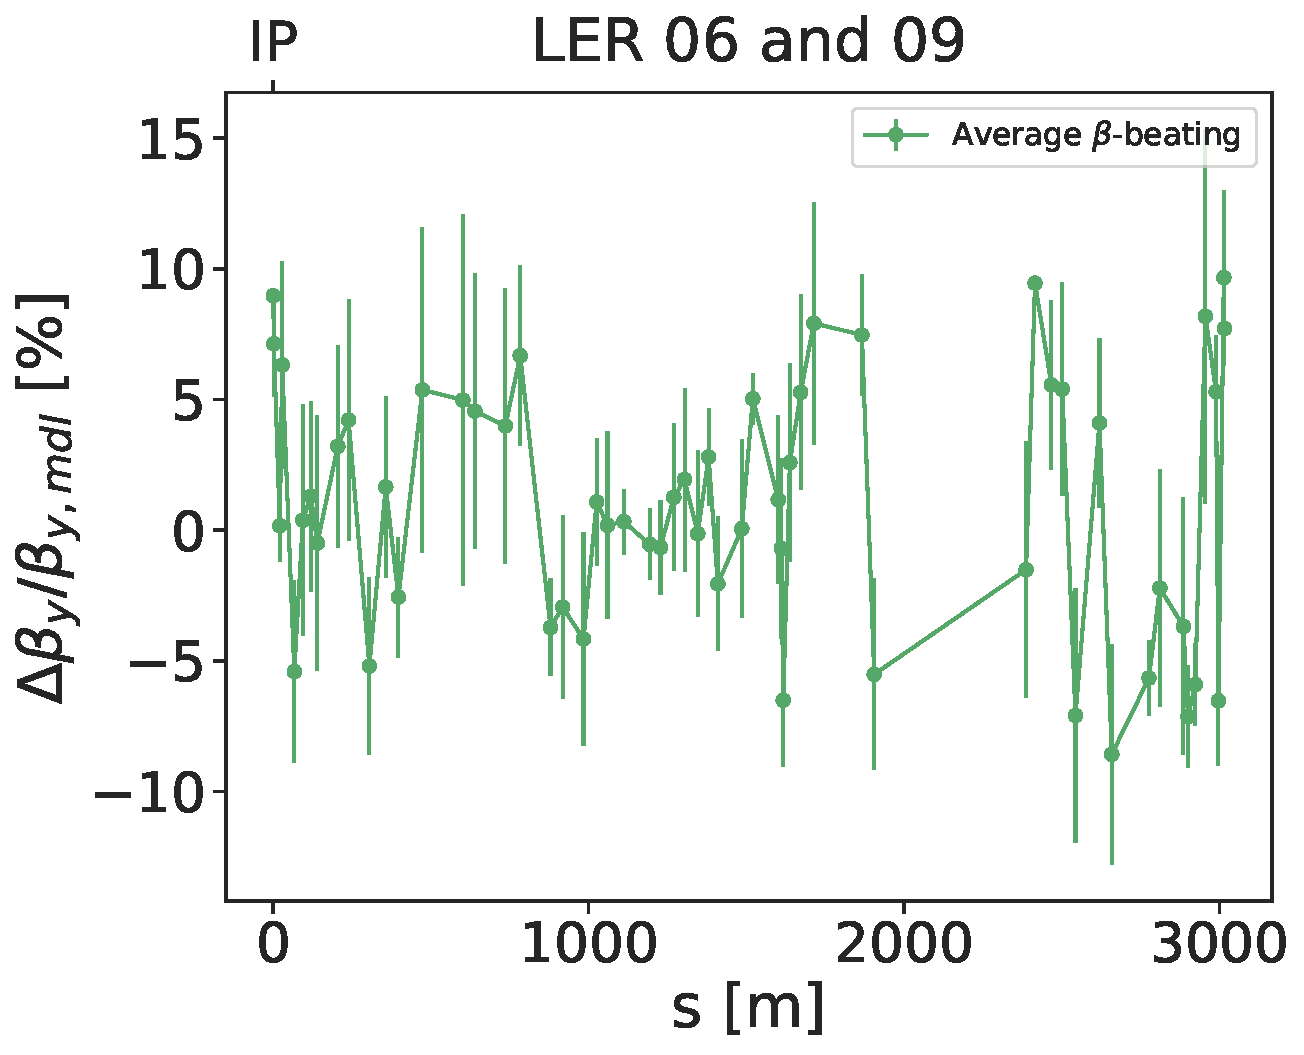
\includegraphics[width=\linewidth]{images/kek/ler_06_09_bet_y.pdf}
        \caption{Vertical beta-beating, RMS is $\approx 4\%$.}
    \end{subfigure}
    \caption{LER horizontal and vertical beta-beating for \textit{detuned} optics, reliably measured
    during two different days.  The vertical plane is noticeably noisier as oscillation amplitudes
    are smaller.}
    \label{fig:kek:beating_ler_detuned}
\end{figure}

action 5 times lower than horizontal

\begin{figure}[!htb]
    \centering
    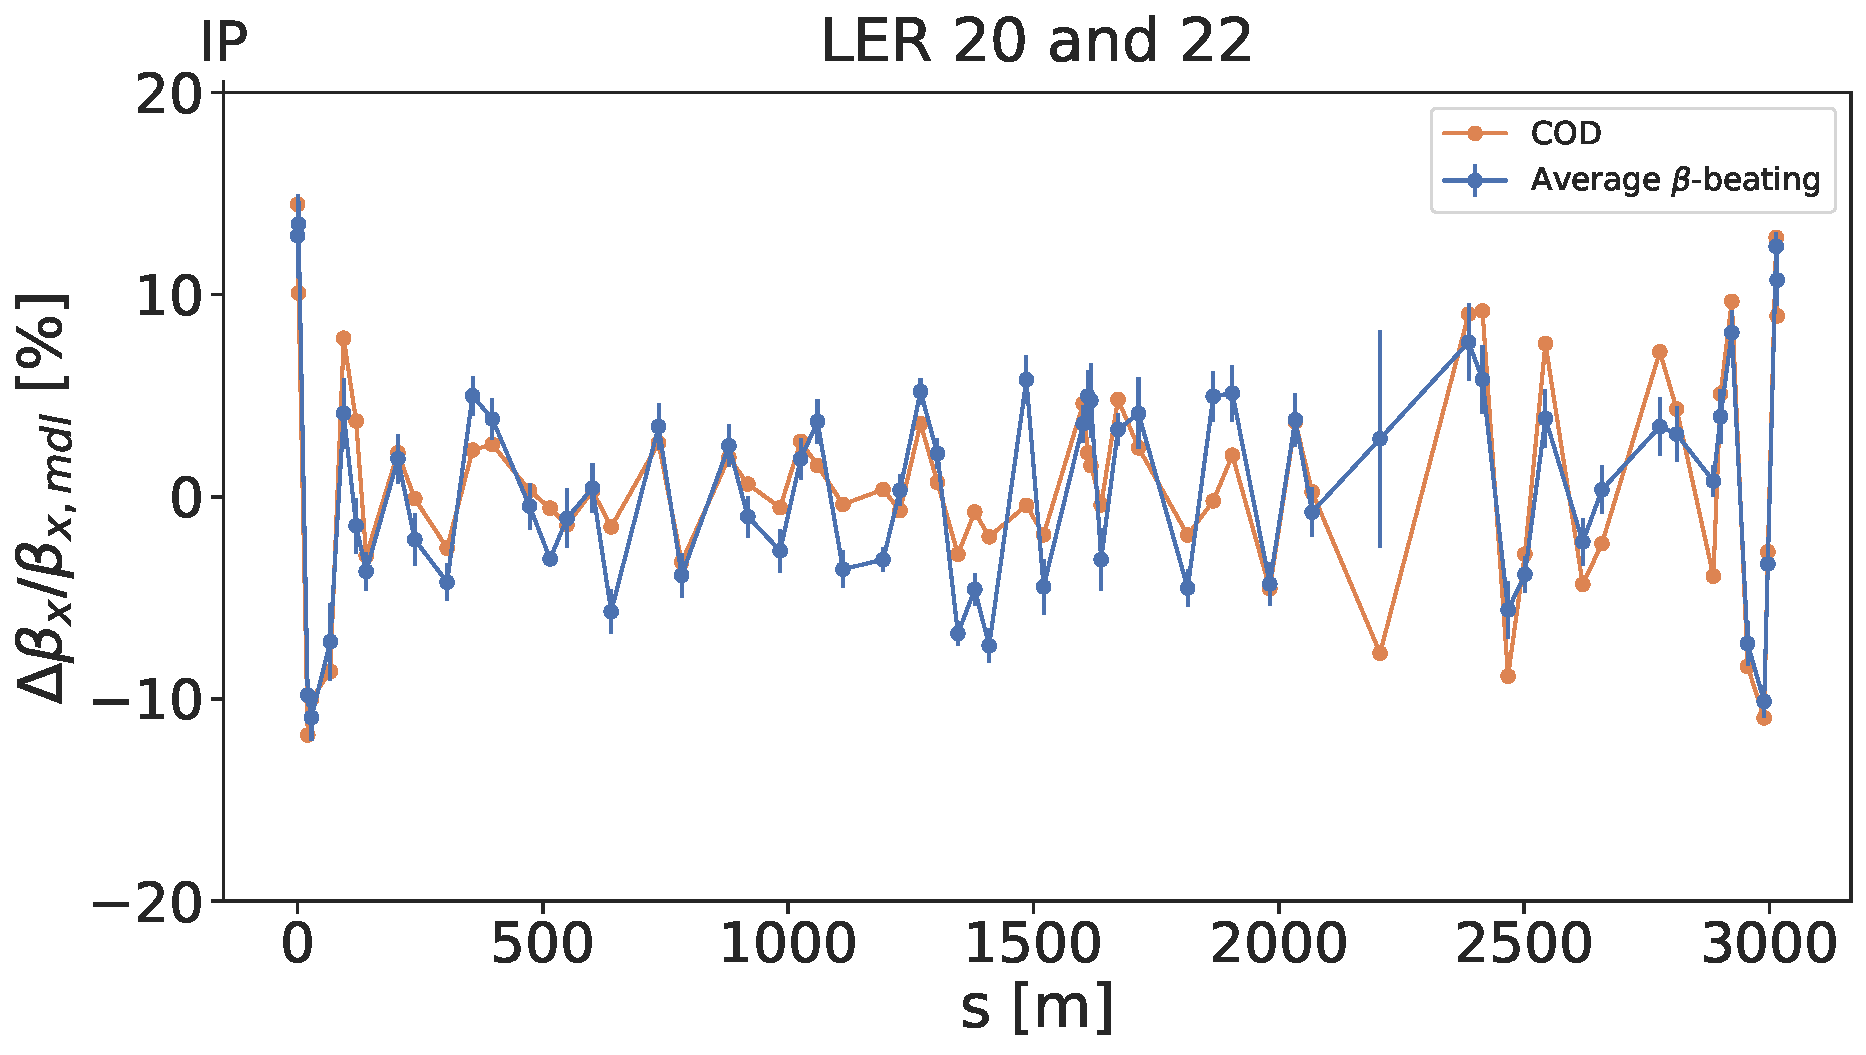
\includegraphics[width=0.7\linewidth]{images/kek/ler_20_22_bet_x.pdf}
    \caption{LER horizontal beta-beating for \textit{8mm squeezed} optics, reliably measured during
    two different days. The vertical plane is absent due to amplitudes being too low to reconstruct
    linear optics. A comparison to the beating measured via LOCO is made.}
    \label{fig:kek:beating_ler_squeezed}
\end{figure}



%-----------------------------
%            HER
\FloatBarrier
\subsubsection{\todo{HER $\beta-beating$}}

\begin{figure}[!htb]
    \centering
    \begin{subfigure}[b]{0.48\textwidth}
        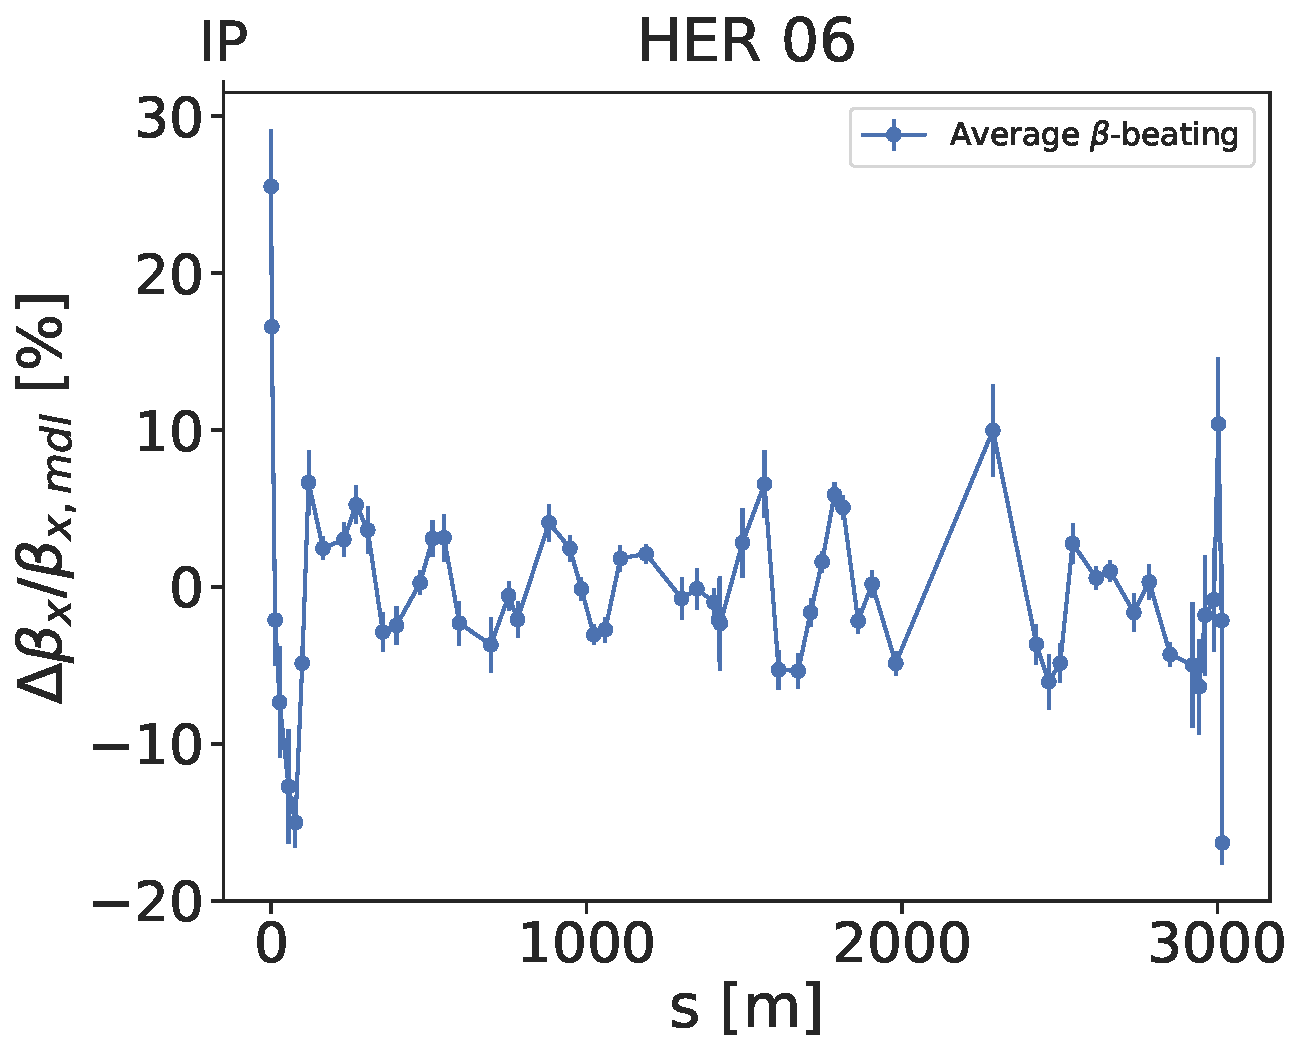
\includegraphics[width=\linewidth]{images/kek/her_06_bet_x.pdf}
        \caption{Horizontal beta-beating, RMS is $\approx 6\%$.}
    \end{subfigure}
    \hfill
    \begin{subfigure}[b]{0.48\textwidth}
        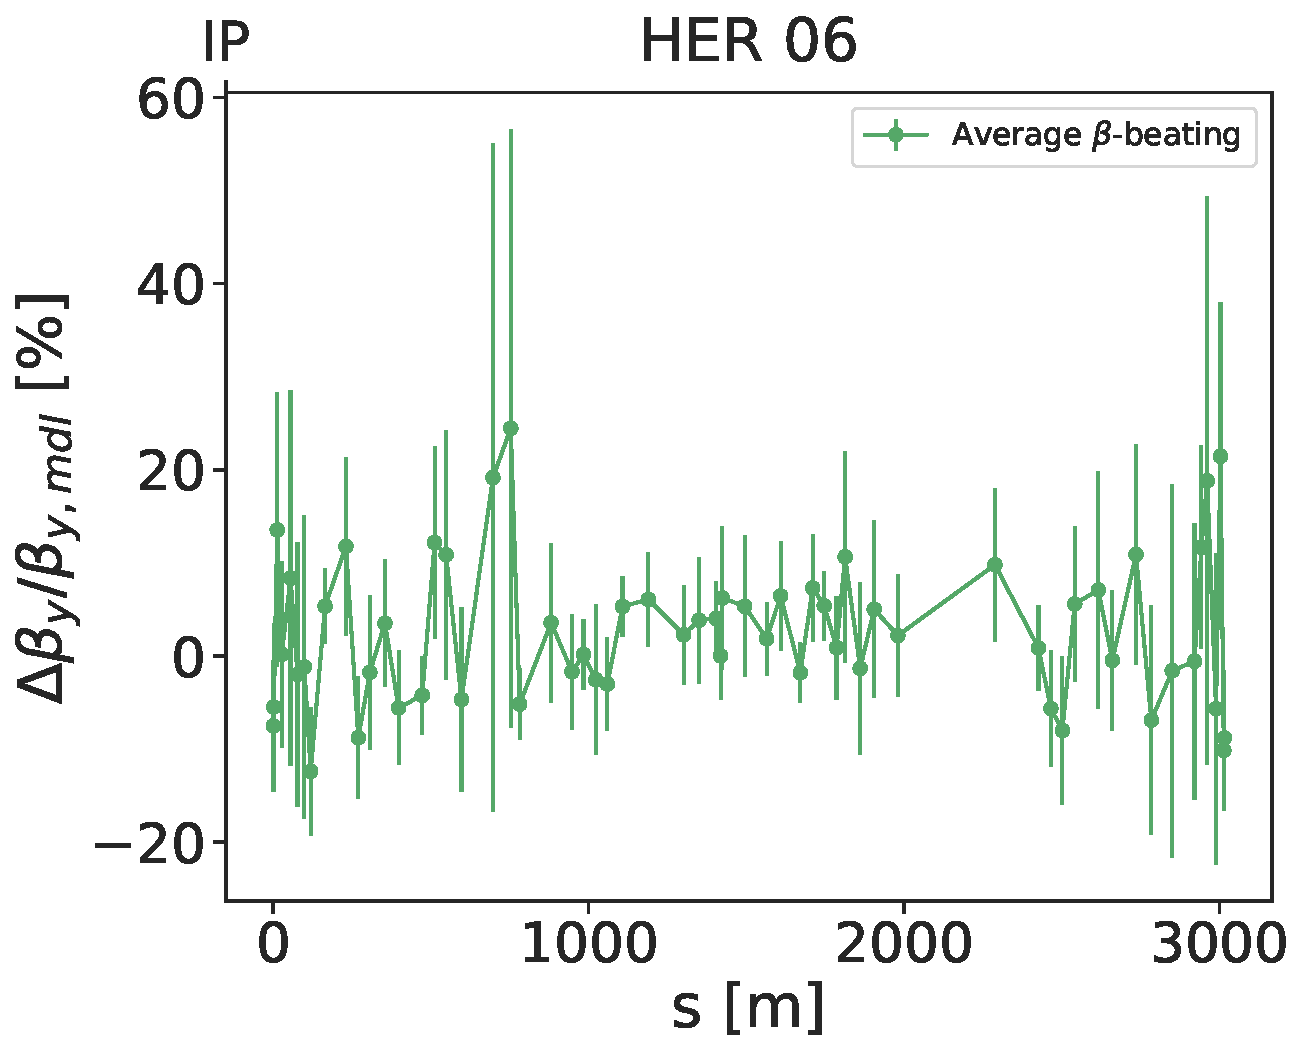
\includegraphics[width=\linewidth]{images/kek/her_06_bet_y.pdf}
        \caption{Vertical beta-beating, RMS is $\approx 8\%$.}
    \end{subfigure}
    \caption{HER horizontal and vertical beta-beating for \textit{detuned} optics. The vertical
    plane is noticeably noisier as oscillation amplitudes are smaller.}
    \label{fig:kek:beating_her_detuned}
\end{figure}

action 5 times lower than H

\begin{figure}[!htb]
    \centering
    \begin{subfigure}[b]{0.48\textwidth}
        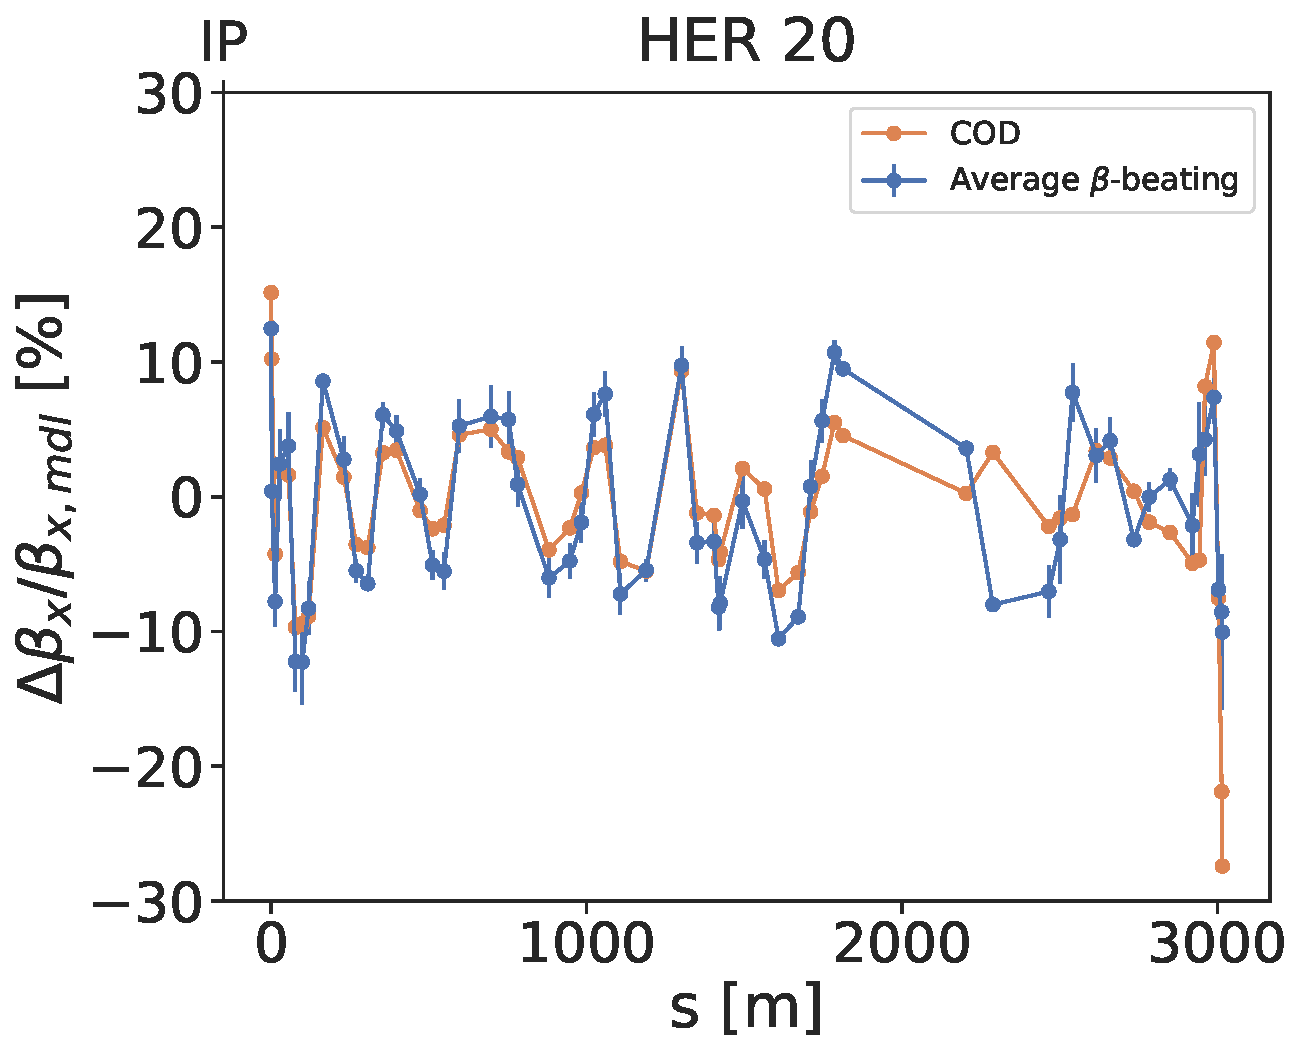
\includegraphics[width=\linewidth]{images/kek/her_20_bet_x_unzoomed.pdf}
        \caption{Horizontal beta-beating, RMS is $\approx 7\%$.}
    \end{subfigure}
    \hfill
    \begin{subfigure}[b]{0.48\textwidth}
        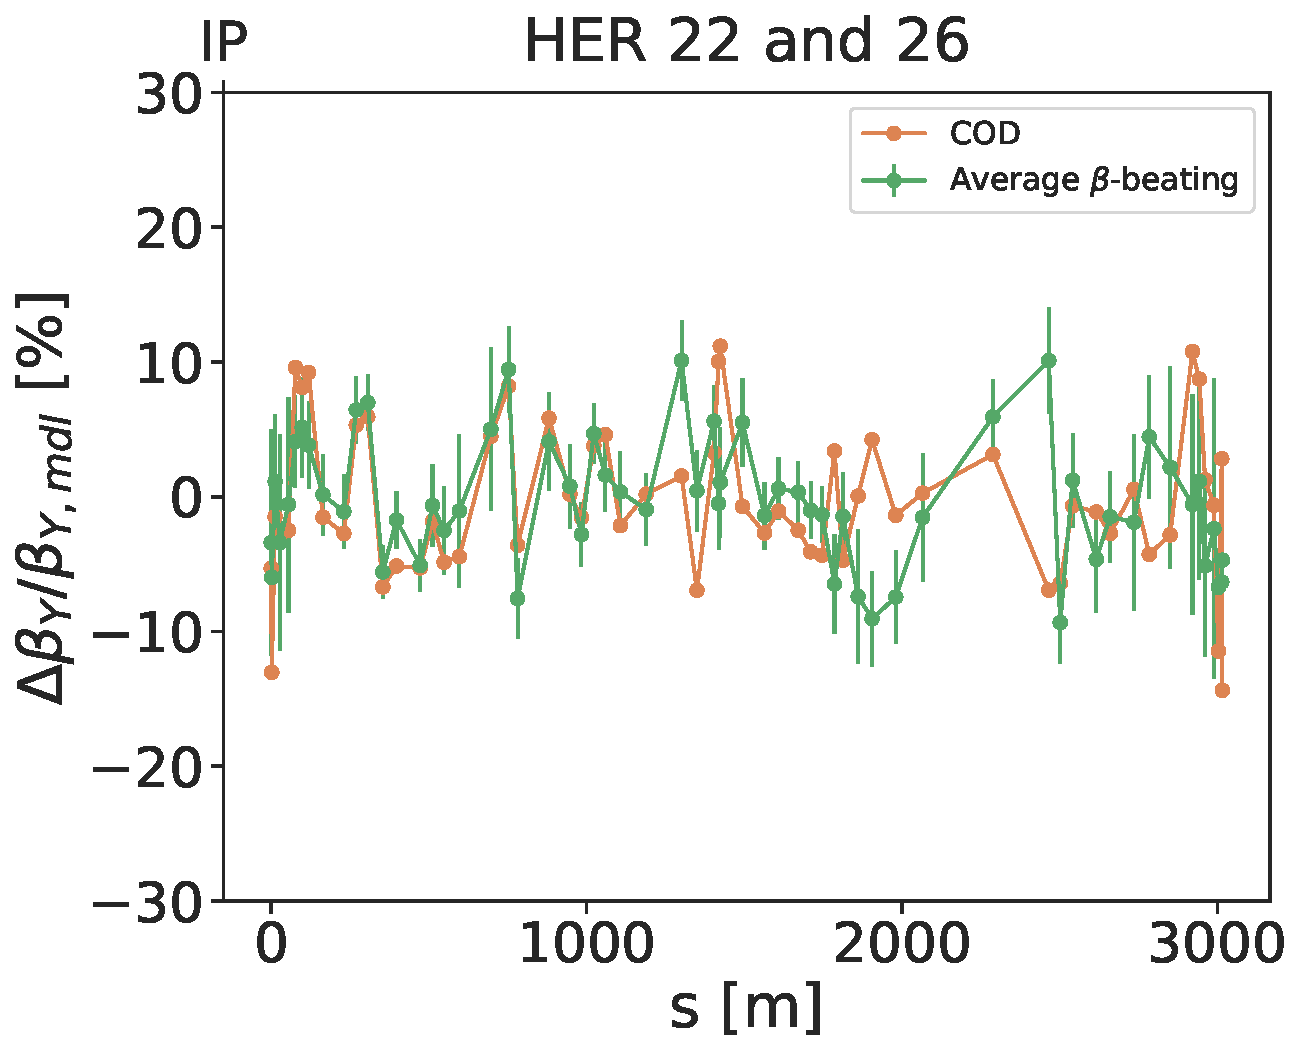
\includegraphics[width=\linewidth]{images/kek/her_22_26_bet_y_unzoomed.pdf}
        \caption{Vertical beta-beating, RMS is $\approx 5\%$.}
    \end{subfigure}
    \caption{HER horizontal and vertical beta-beating for \textit{8mm squeezed} optics. The vertical
    plane is noticeably noisier as oscillation amplitudes are smaller. A comparison to the beating
    measured via LOCO is made.}
    \label{fig:kek:beating_her_squeezed}
\end{figure}


%-----------------------------
%            Summary
\FloatBarrier
\subsubsection{\todo{Summary}}

\begin{table}
    \centering
    \begin{tabular}{llrr}
        \toprule
        Ring & Configuration & $\beta$-b. rms H & $\beta$-b. rms V \\
        \midrule
        LER  &  Detuned      & 4\%              & 5\%   \\
            &  Squeezed 8mm & 6\%              &       \\
        HER  &  Detuned      & 6\%              & 8\%  \\
            &  Squeezed 8mm & 7\%              & 5\%  \\
        \bottomrule
    \end{tabular}
    \caption{Summary of the measured $\beta$-beating with squeezed and detuned optics in the HER
    and LER rings.}
    \label{tab:kek:summary_beating}
\end{table}



%-----------------------------
%         LER Amp.Det.
%-----------------------------
\FloatBarrier
\subsection{\todo{Amplitude Detuning}}

%-----------------------------
%         Tune Stability
\FloatBarrier
\subsubsection{\todo{Tune Stability}}


\begin{figure}[!htb]
    \centering
    \begin{subfigure}[b]{0.8\textwidth}
        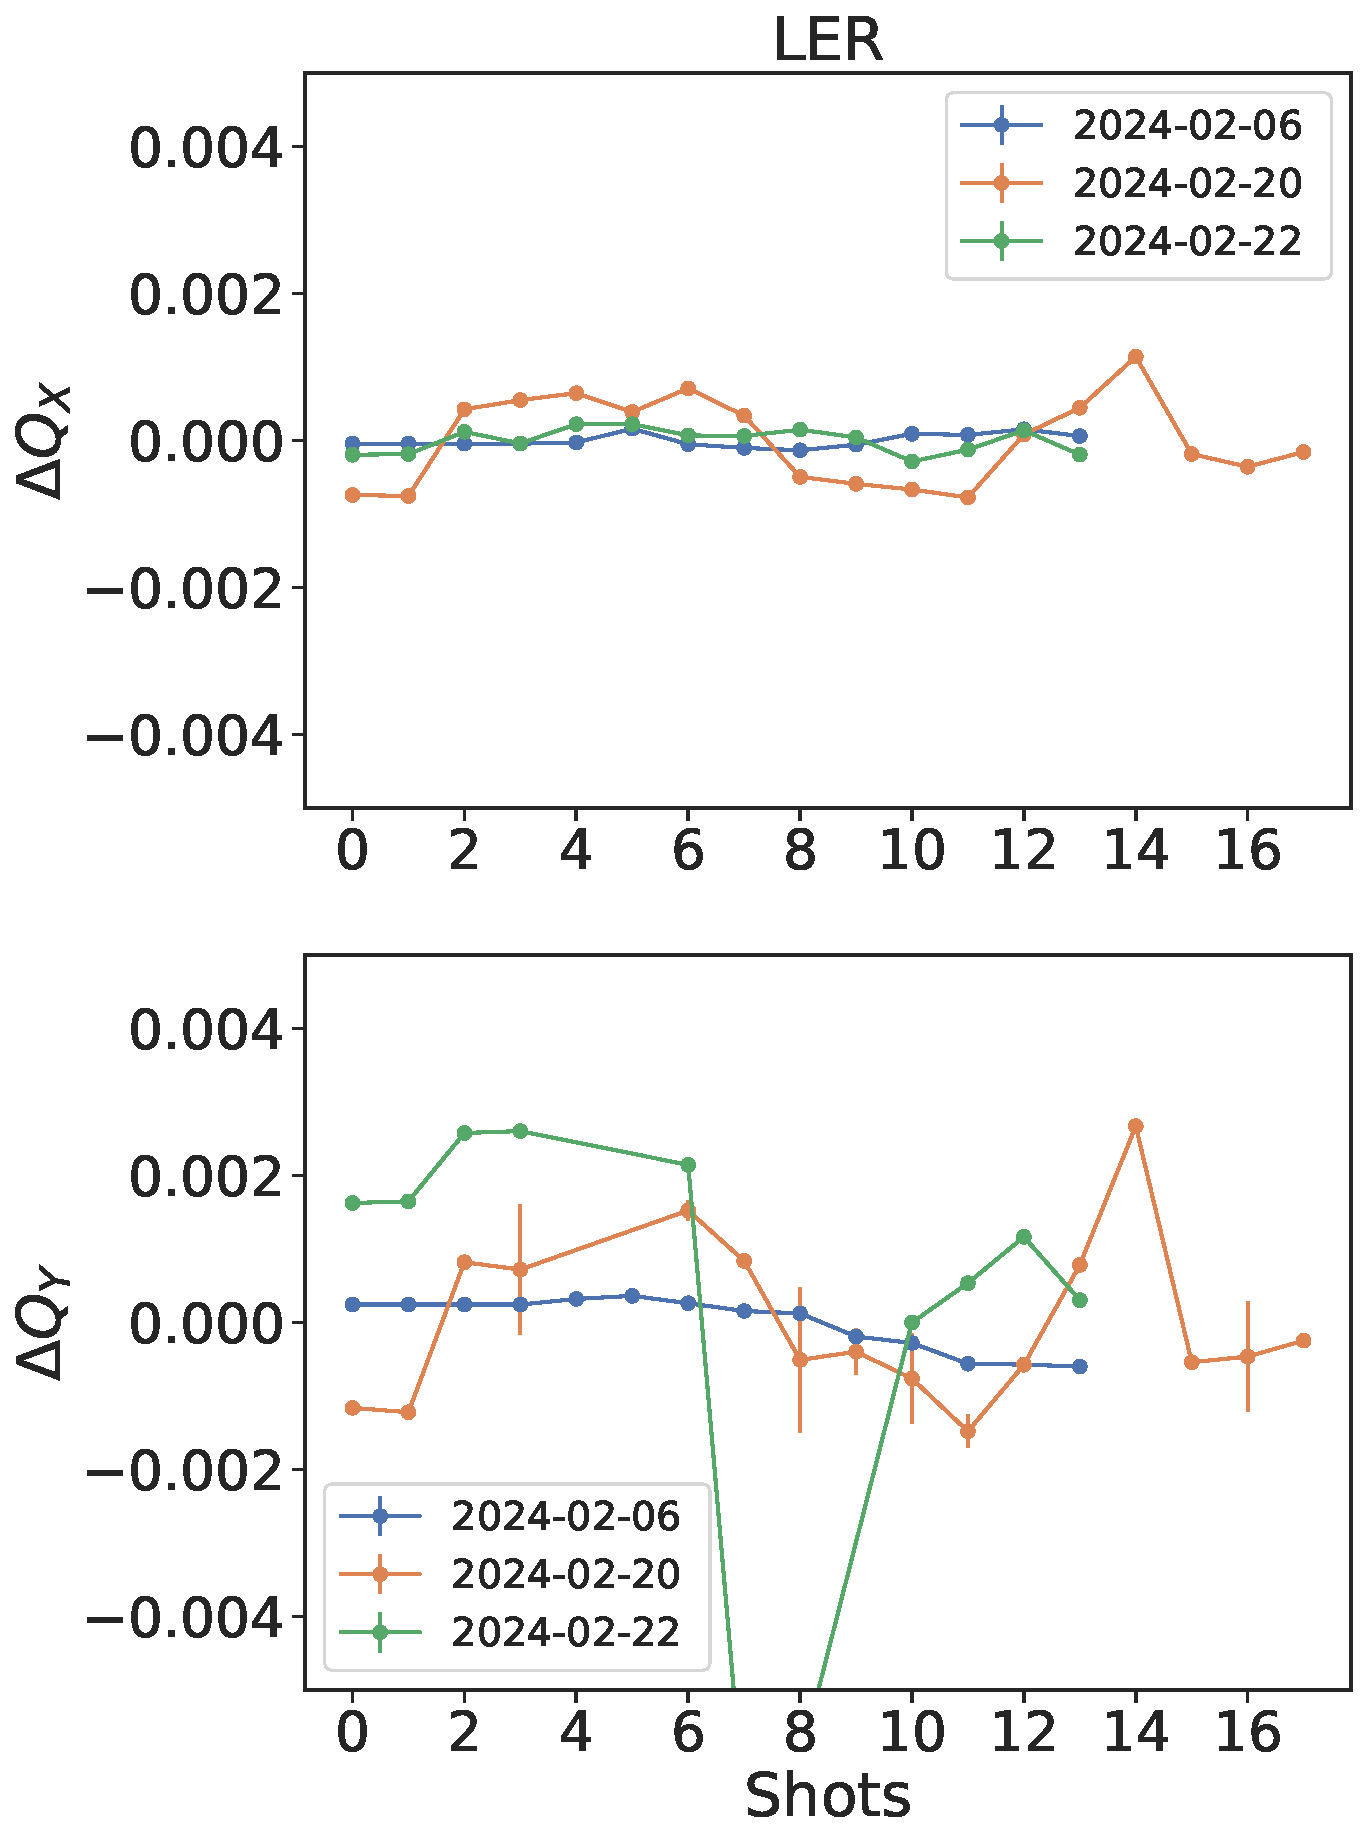
\includegraphics[width=\linewidth]{images/kek/SUPERKEKBLER_shots.pdf}
        \caption{Tune stability for the LER ring.}
    \end{subfigure}
    \vspace{0.5cm} 
    \begin{subfigure}[b]{0.8\textwidth}
        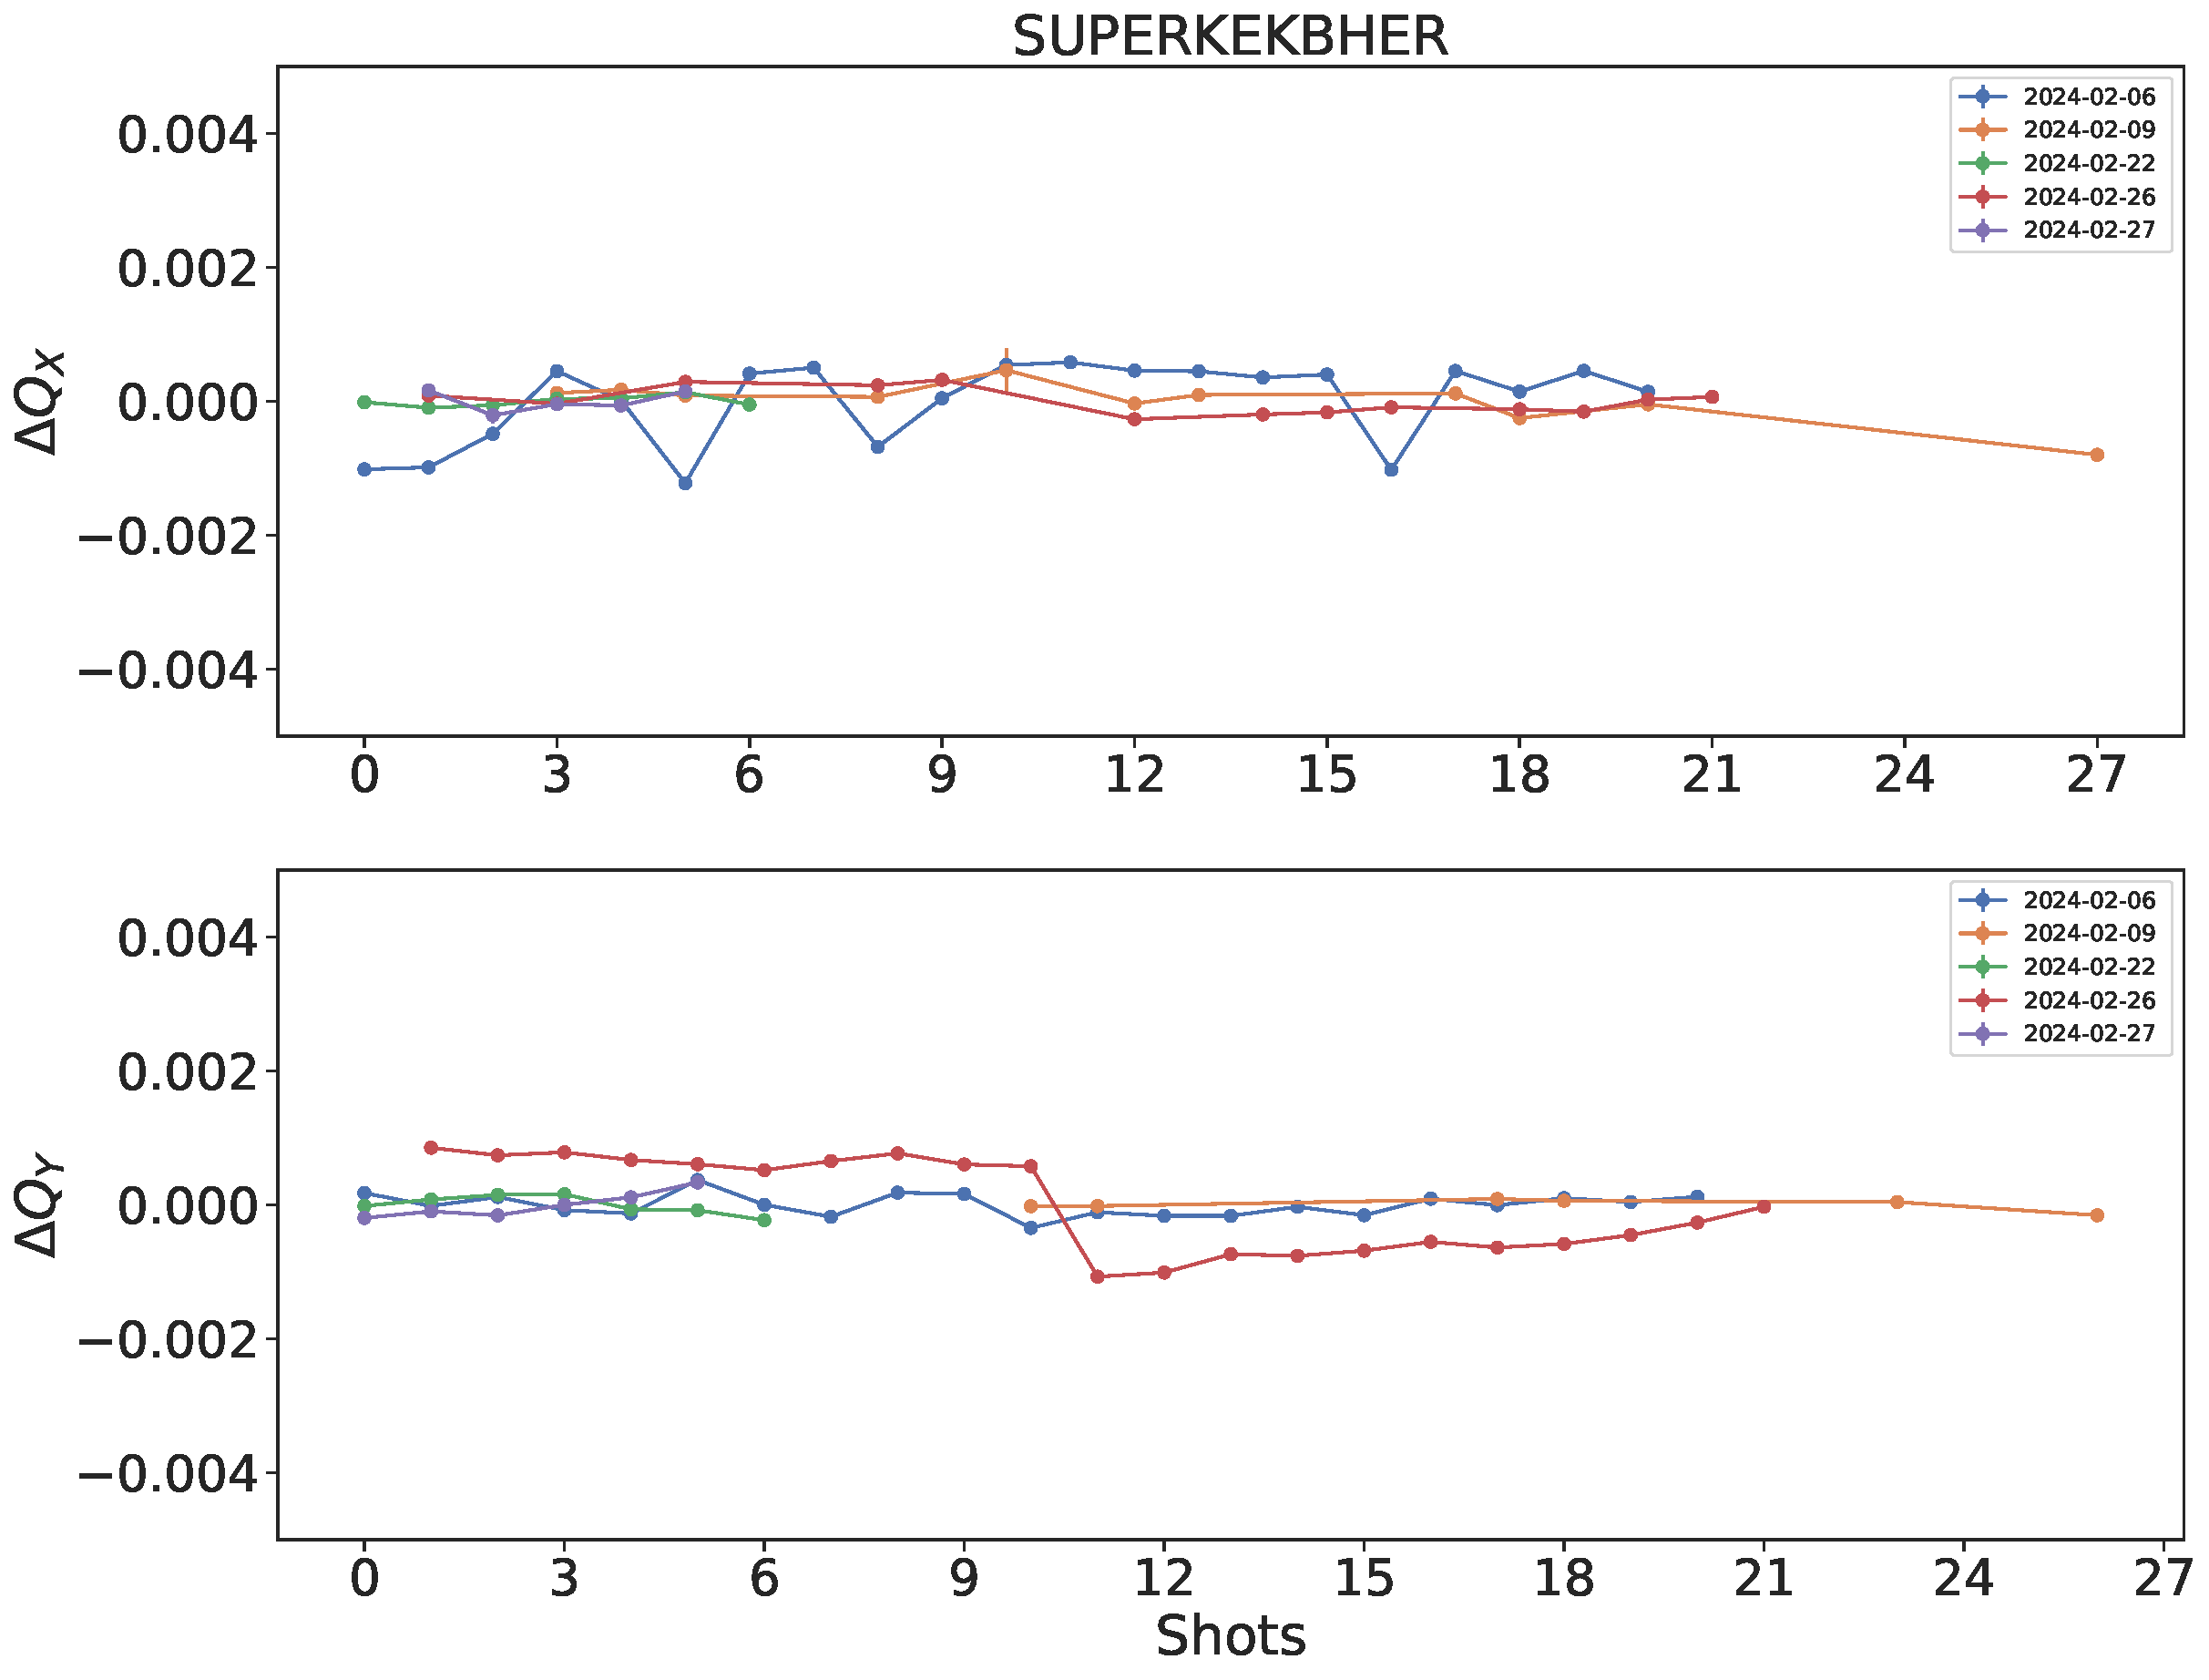
\includegraphics[width=\linewidth]{images/kek/SUPERKEKBHER_shots.pdf}
        \caption{Tune stability for the HER ring.}
    \end{subfigure}
    \caption{Difference in tune between consecutive measurements, across several days.}
    \label{fig:kek:shots}
\end{figure}


%-----------------------------
%             LER
\FloatBarrier
\subsubsection{\todo{Amplitude Detuning in LER}}

\begin{figure}[!htb]
    \centering
    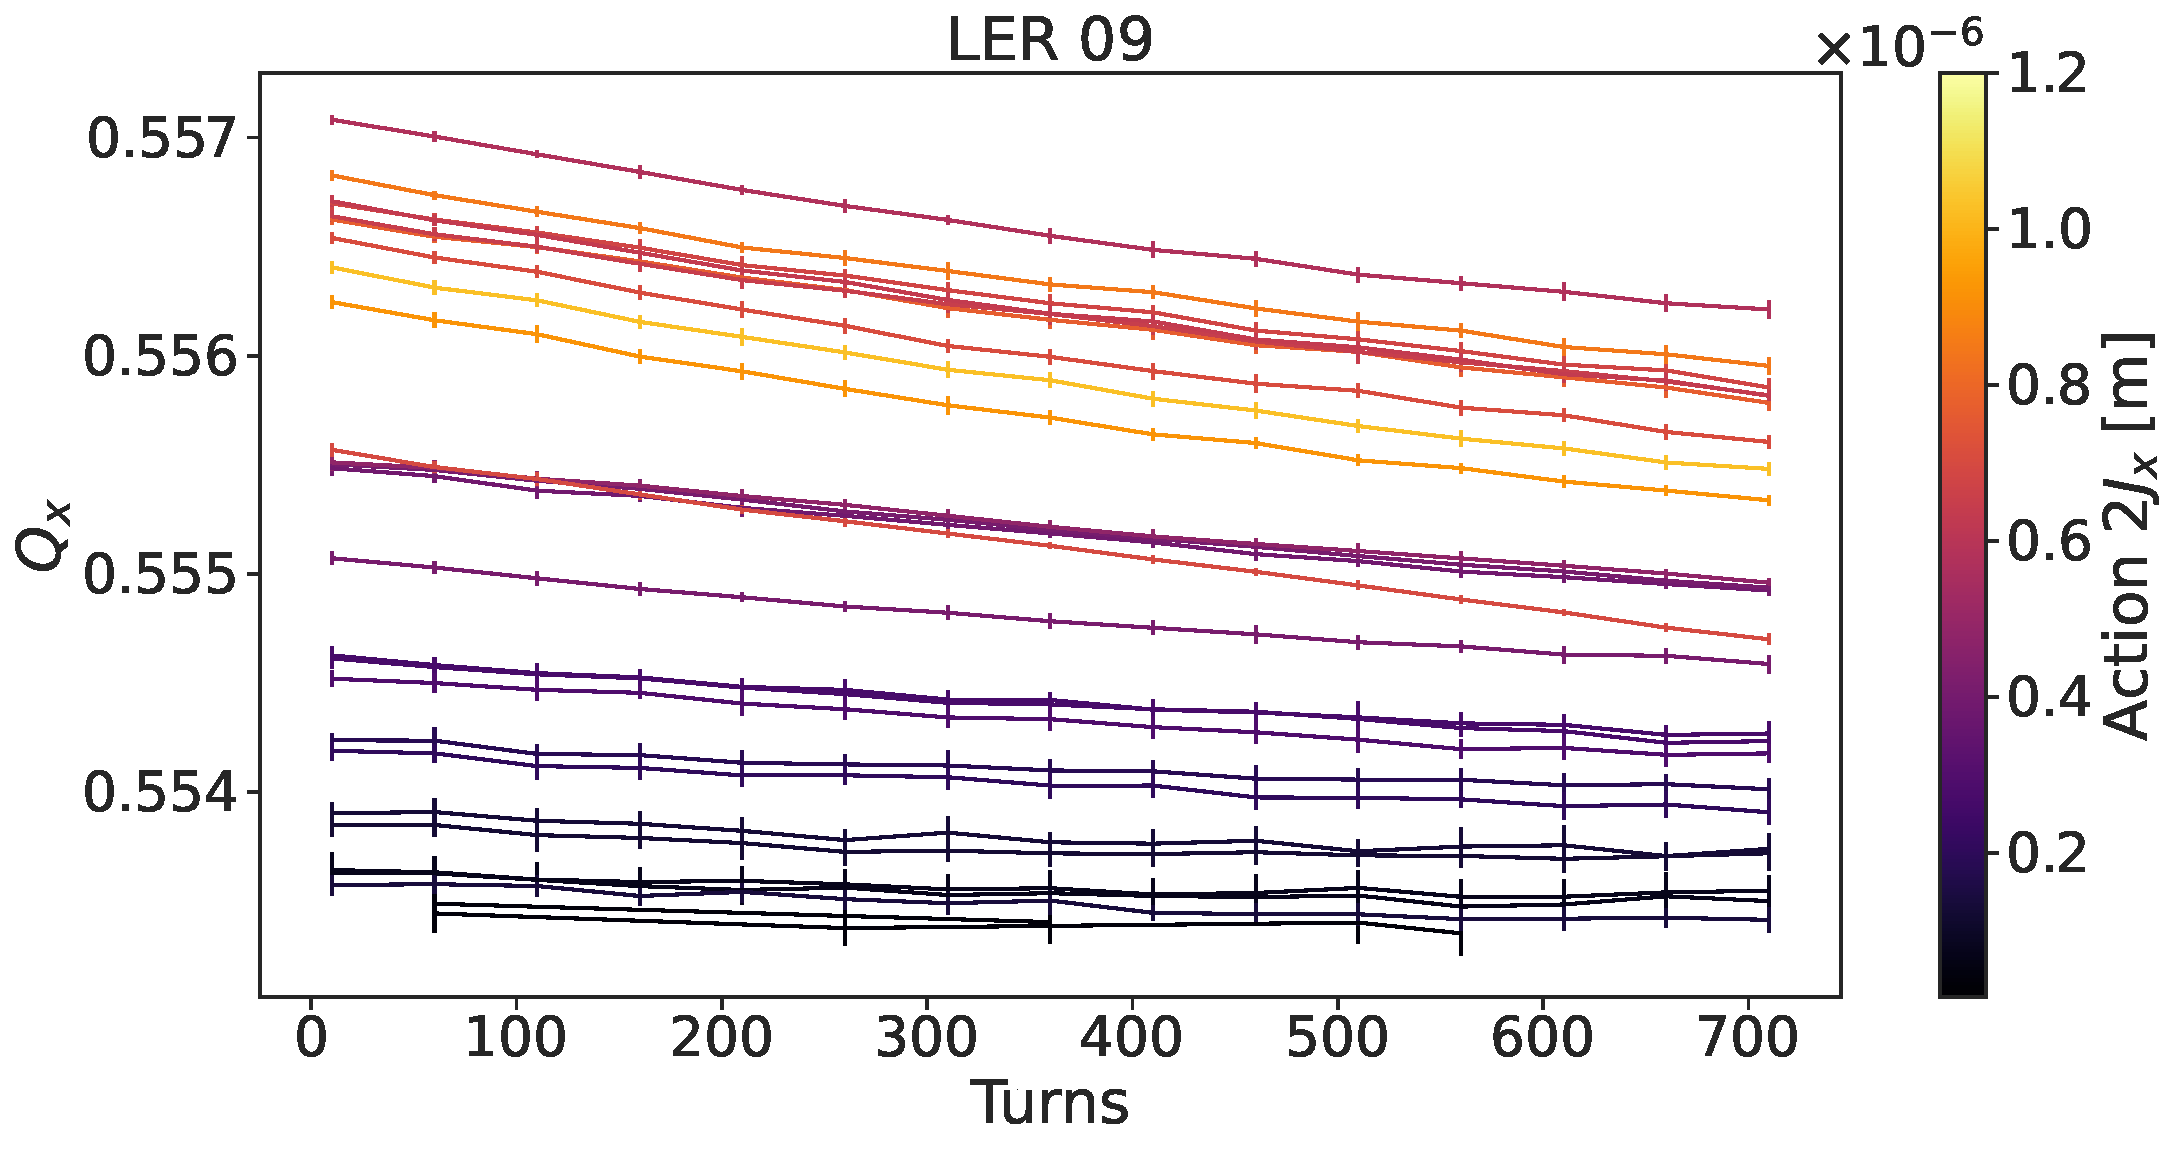
\includegraphics[width=\linewidth]{images/kek/LER_detuned_ampdet.pdf}
    \caption{Correlation between the measured tune with the action of the kick. The tune is computed
    via a running window over 200 turns, every 50 turns.}
    \label{fig:kek:ler_full_tune_ampdet}
\end{figure}



\begin{figure}[!htb]
    \centering
    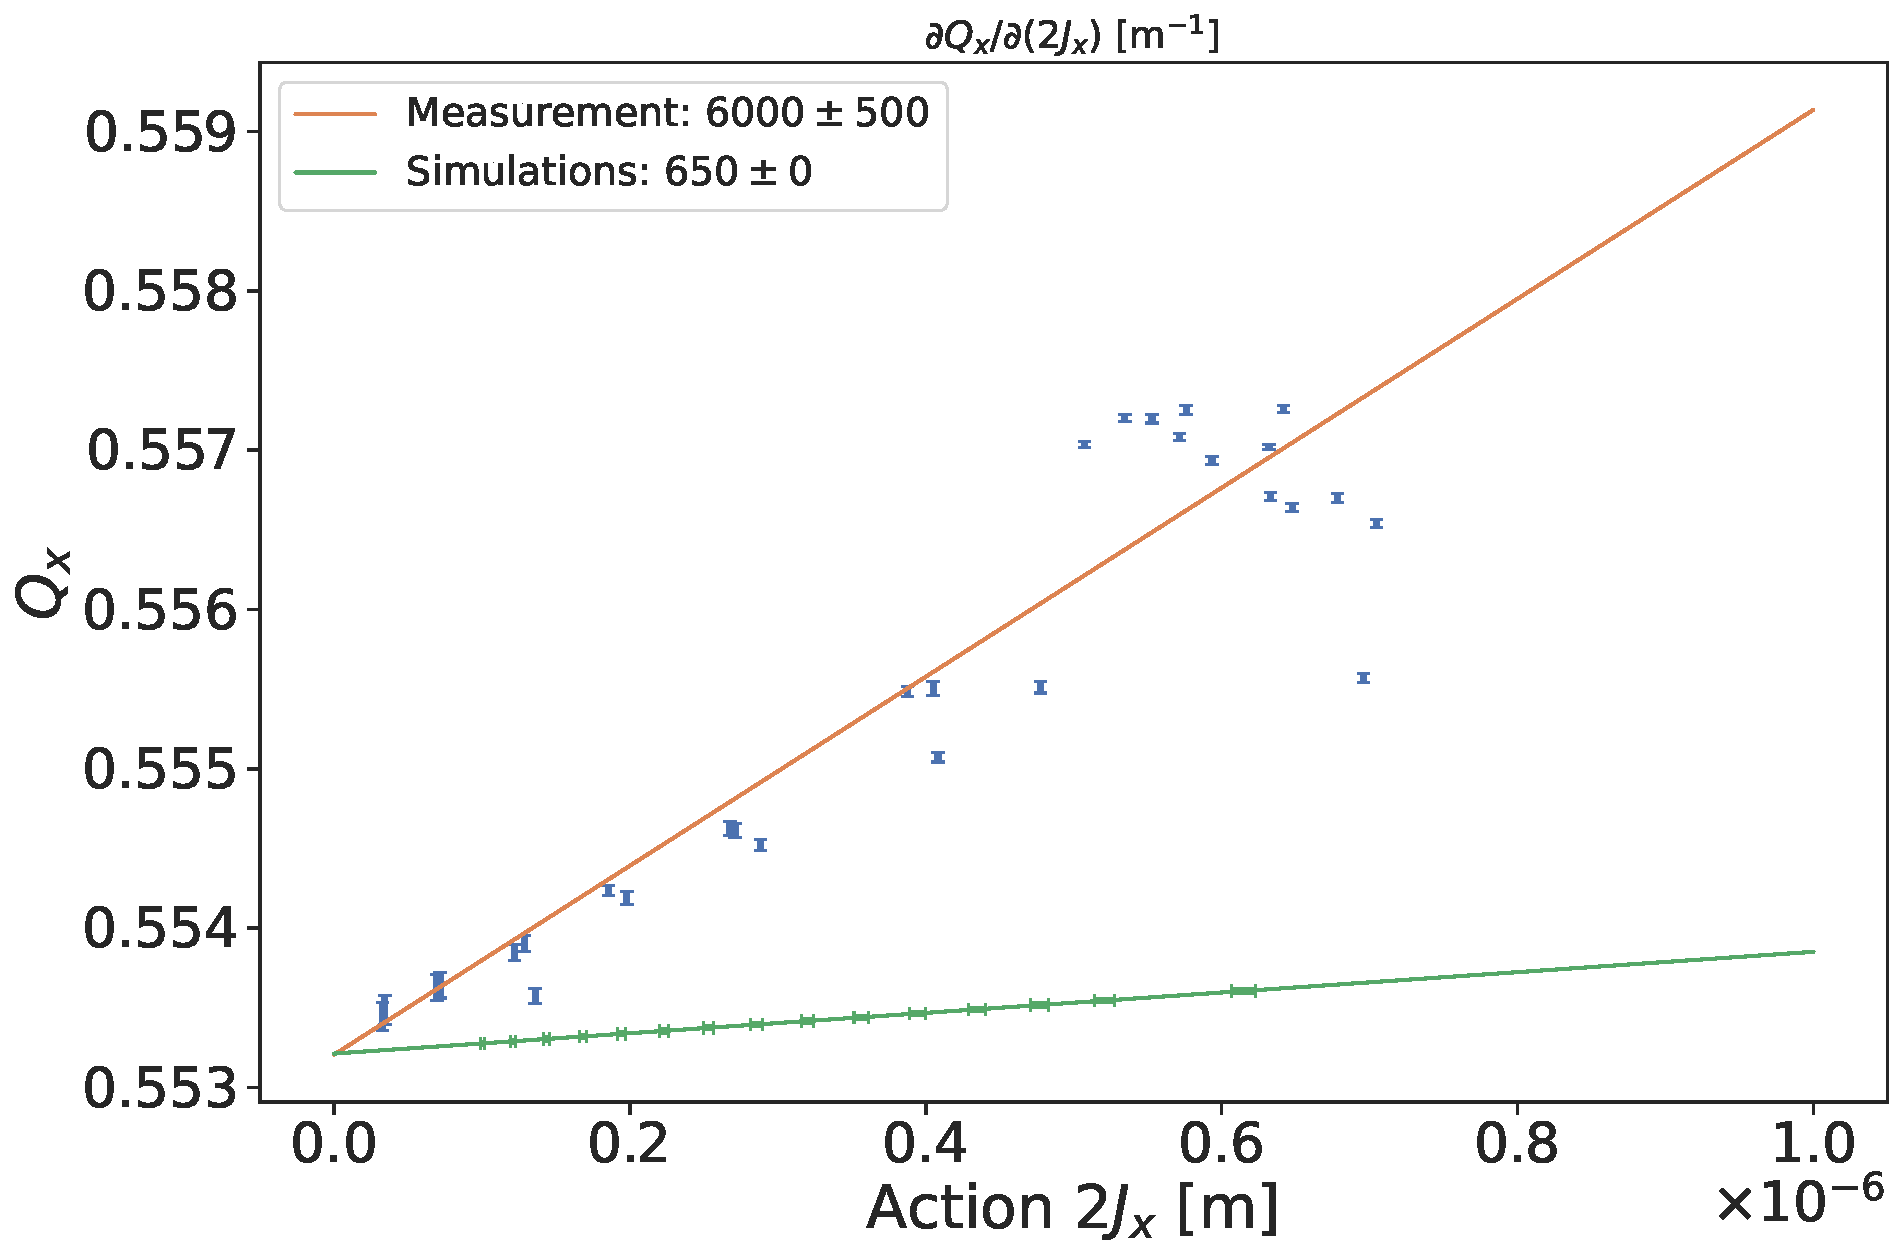
\includegraphics[width=0.9\linewidth]{images/kek/amplitude_detuning.pdf}
    \caption{Amplitude dependence of the tune in the LER ring. The fitted line then corresponds to
    the amplitude detuning term $\partial Q_x/\partial 2J_x$. For comparison, the model computed 
    from the model is shown in green.}
    \label{fig:kek:ler_ampdet}
\end{figure}



%-----------------------------
%   Resonance Driving Terms
%-----------------------------
\FloatBarrier
\subsection{\todo{Resonance Driving Terms}}

\begin{figure}[!htb]
    \centering
    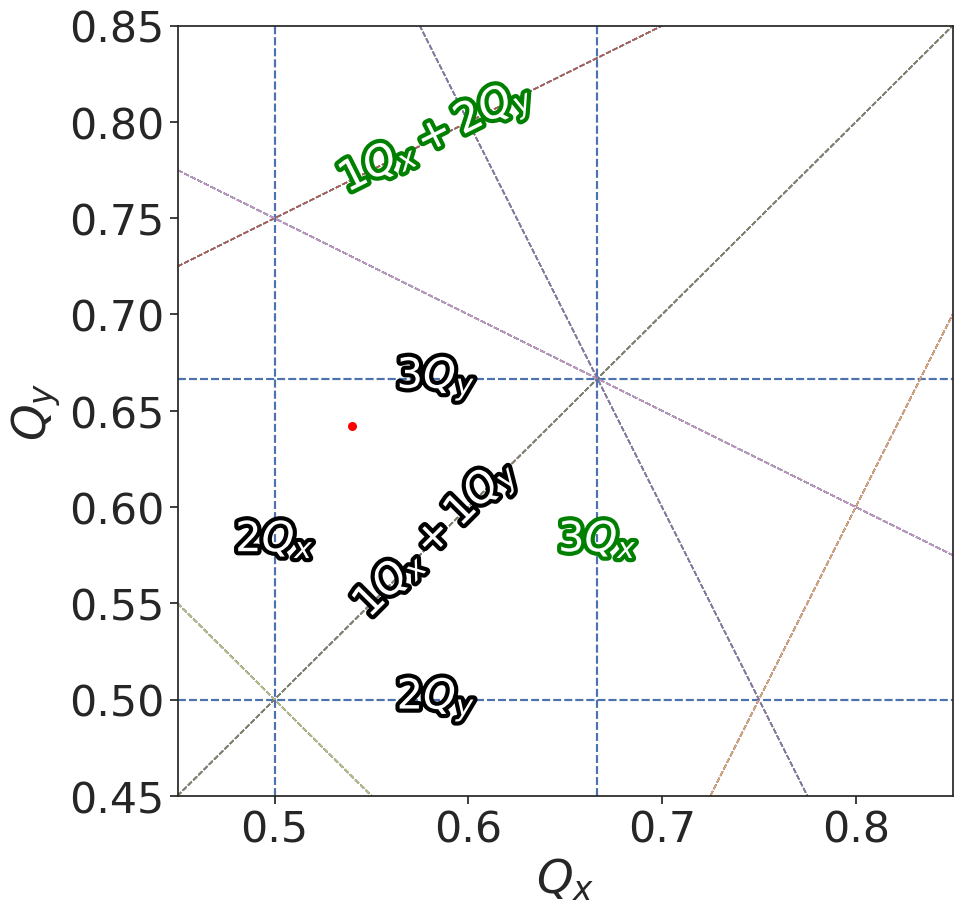
\includegraphics[width=0.6\linewidth]{images/kek/tune_diagram.png}
    \caption{}
    \label{fig:kek:tune_diagram}
\end{figure}

\begin{figure}[!htb]
    \centering
    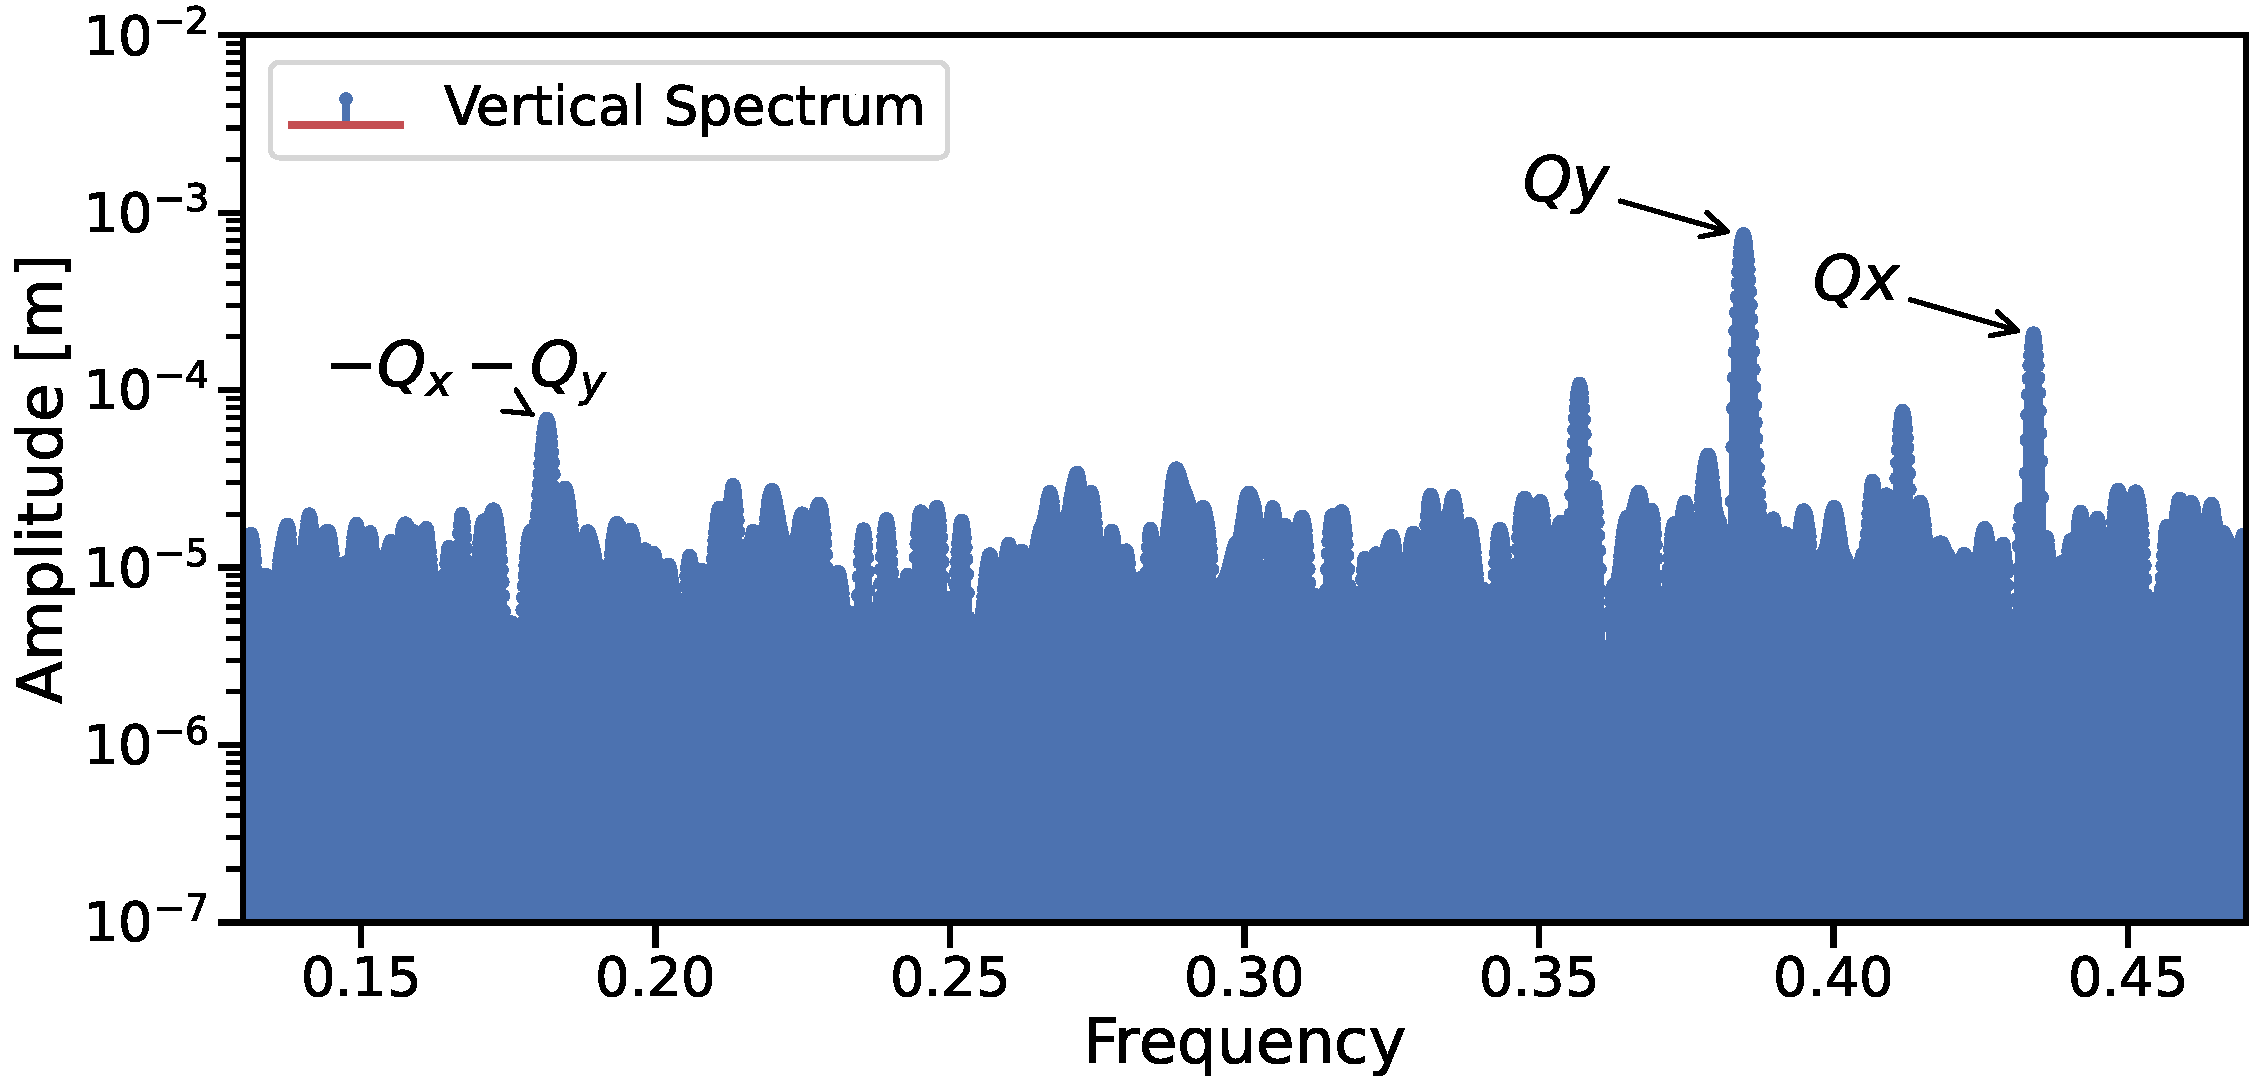
\includegraphics[width=\linewidth]{images/kek/HER_2024-02-06_sextupoles_spectrum.pdf}
    \caption{}
    \label{fig:kek:rdt_spectrum_HER}
\end{figure}

\begin{figure}[!htb]
    \centering
    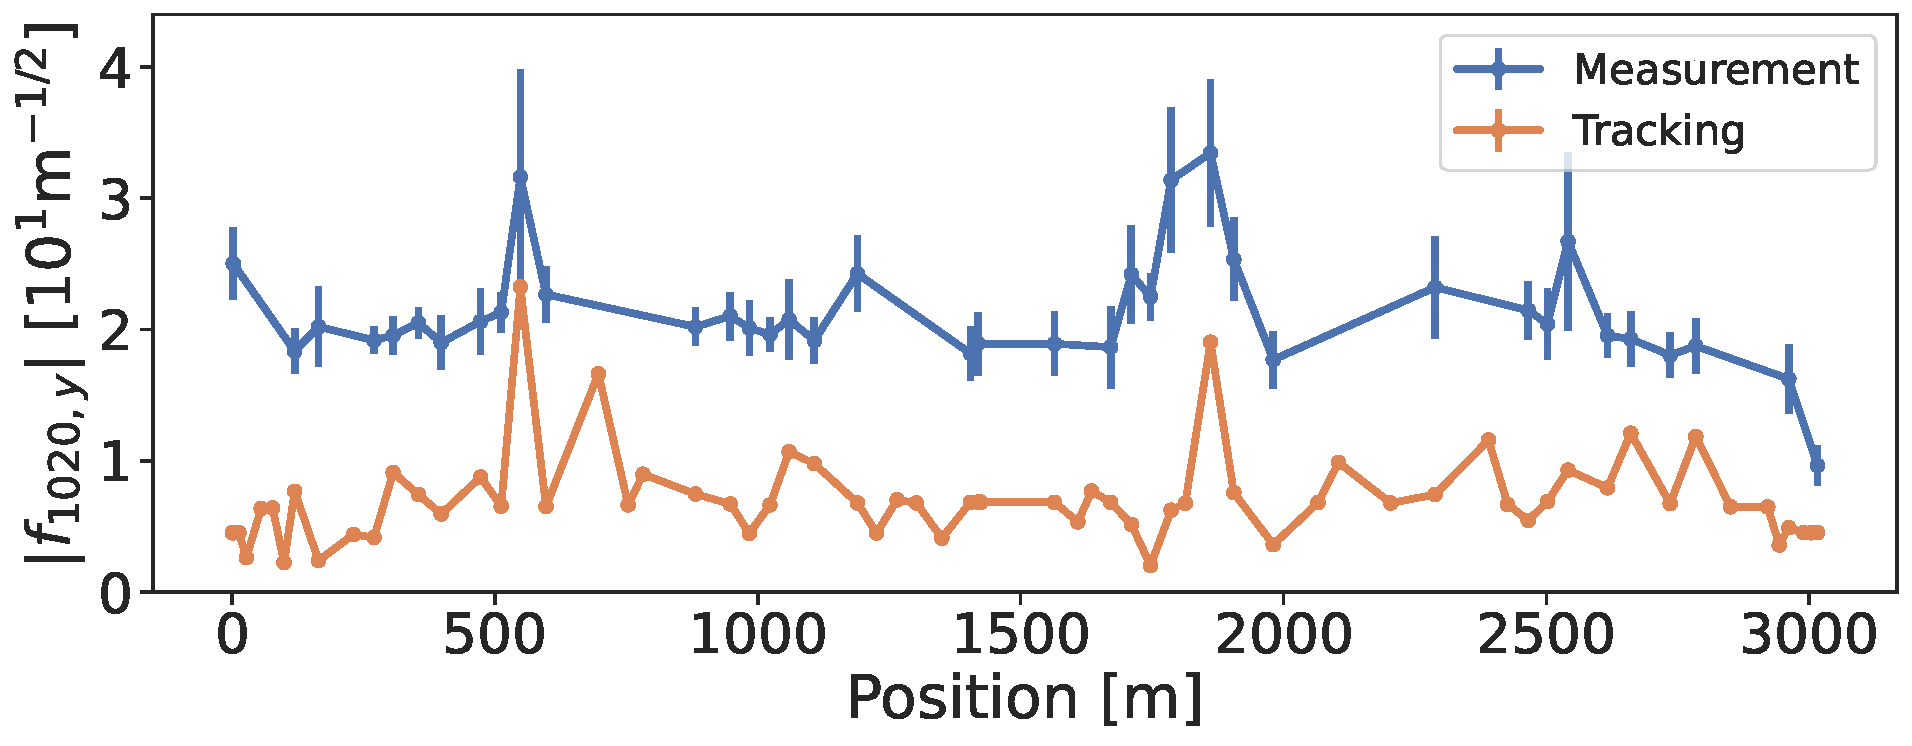
\includegraphics[width=0.8\linewidth]{images/kek/f1020y_HER.pdf}
    \caption{}
    \label{fig:kek:rdt_f1020y_HER}
\end{figure}

\begin{figure}[!htb]
    \centering
    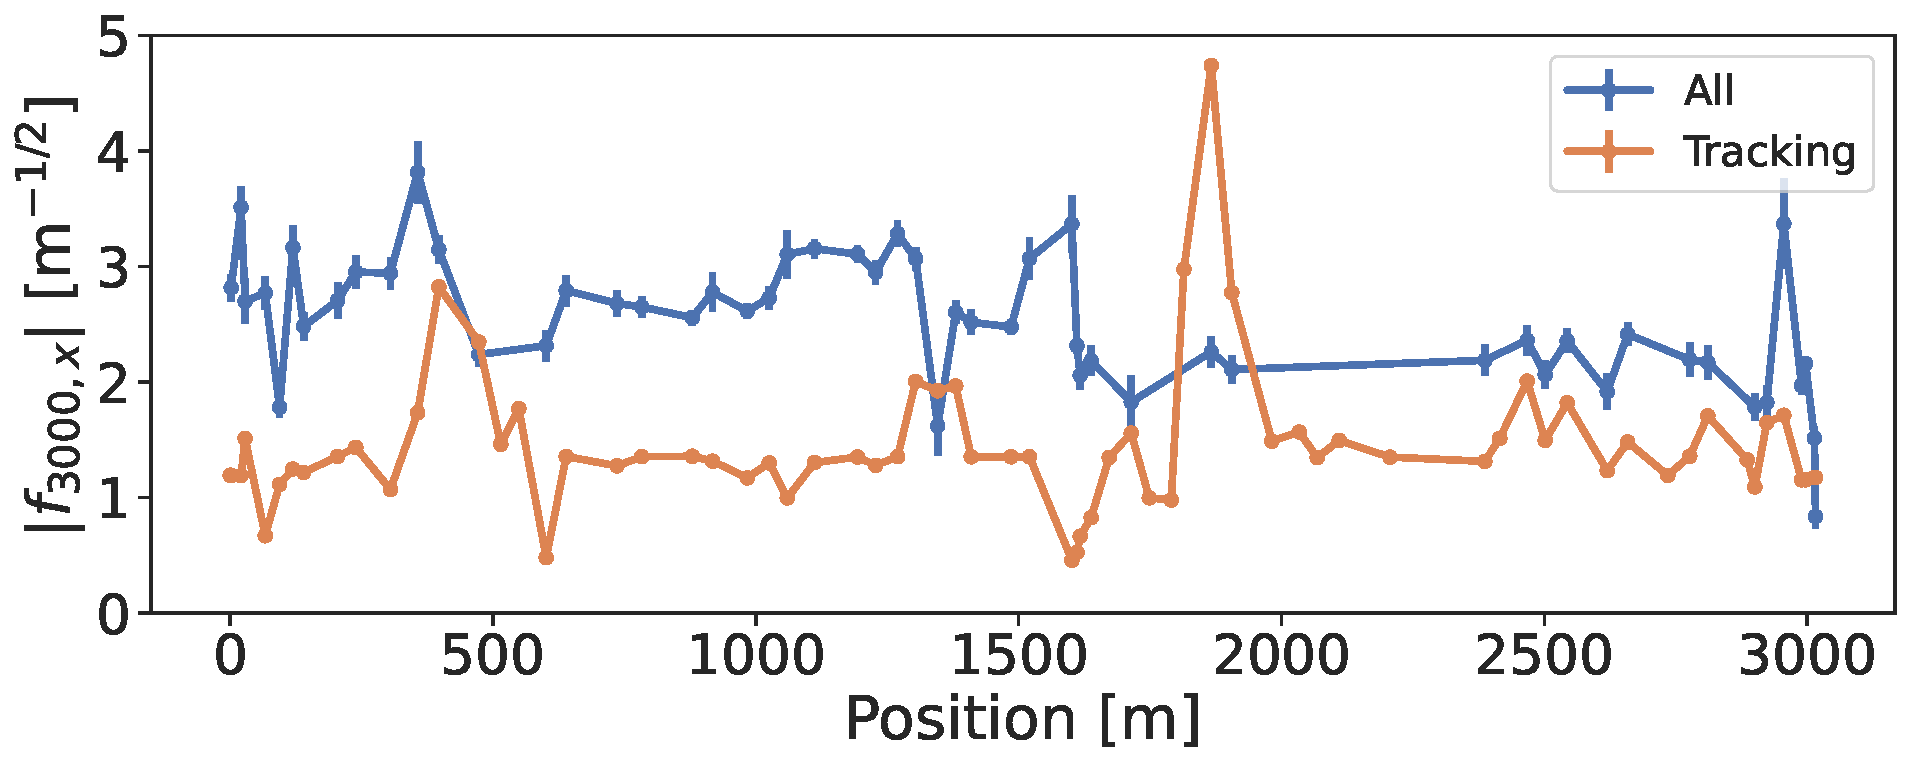
\includegraphics[width=0.8\linewidth]{images/kek/f3000x_LER.pdf}
    \caption{}
    \label{fig:kek:rdt_f3000x_LER}
\end{figure}



%-----------------------------
%        Chromaticity
%-----------------------------
\FloatBarrier
\subsection{\todo{Chromaticity}}

\begin{figure}[!htb]
    \centering
    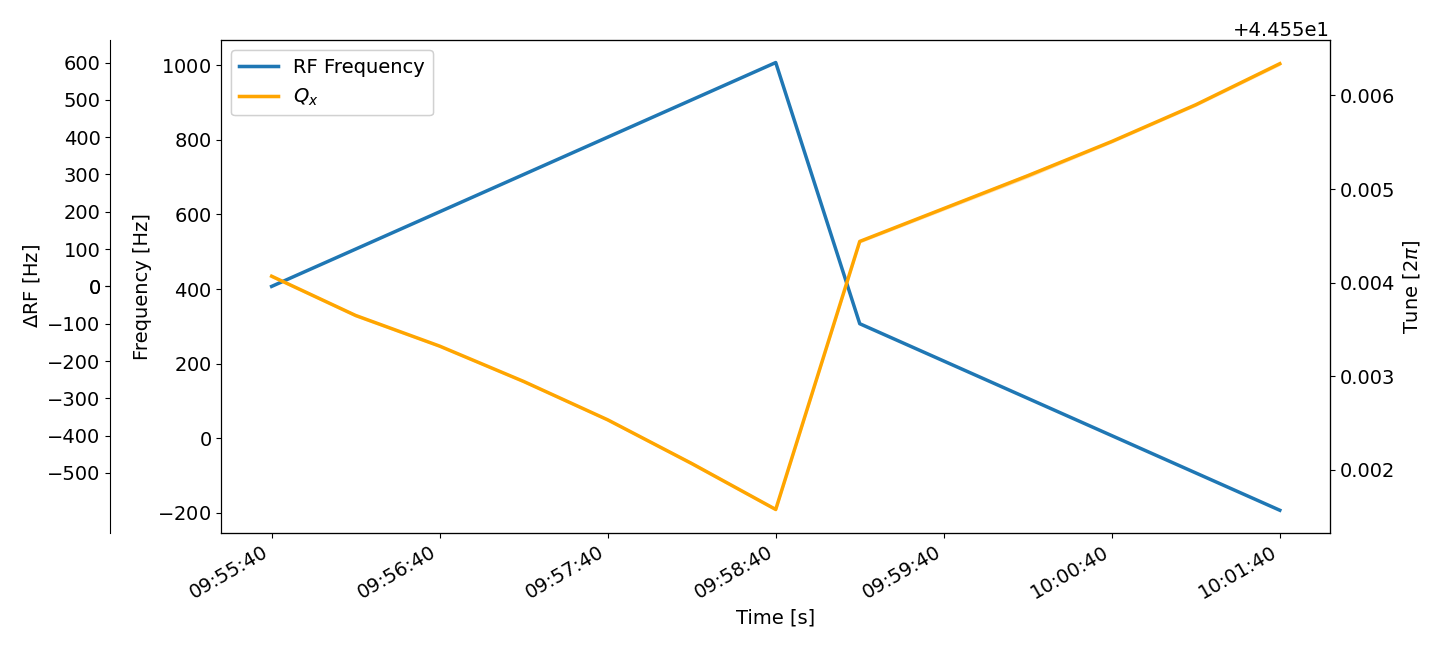
\includegraphics[width=\linewidth]{images/kek/rf_qx.png}
    \caption{}
    \label{fig:kek:chroma_procedure}
\end{figure}


\begin{figure}[!htb]
    \centering
    \begin{subfigure}[b]{0.49\textwidth}
        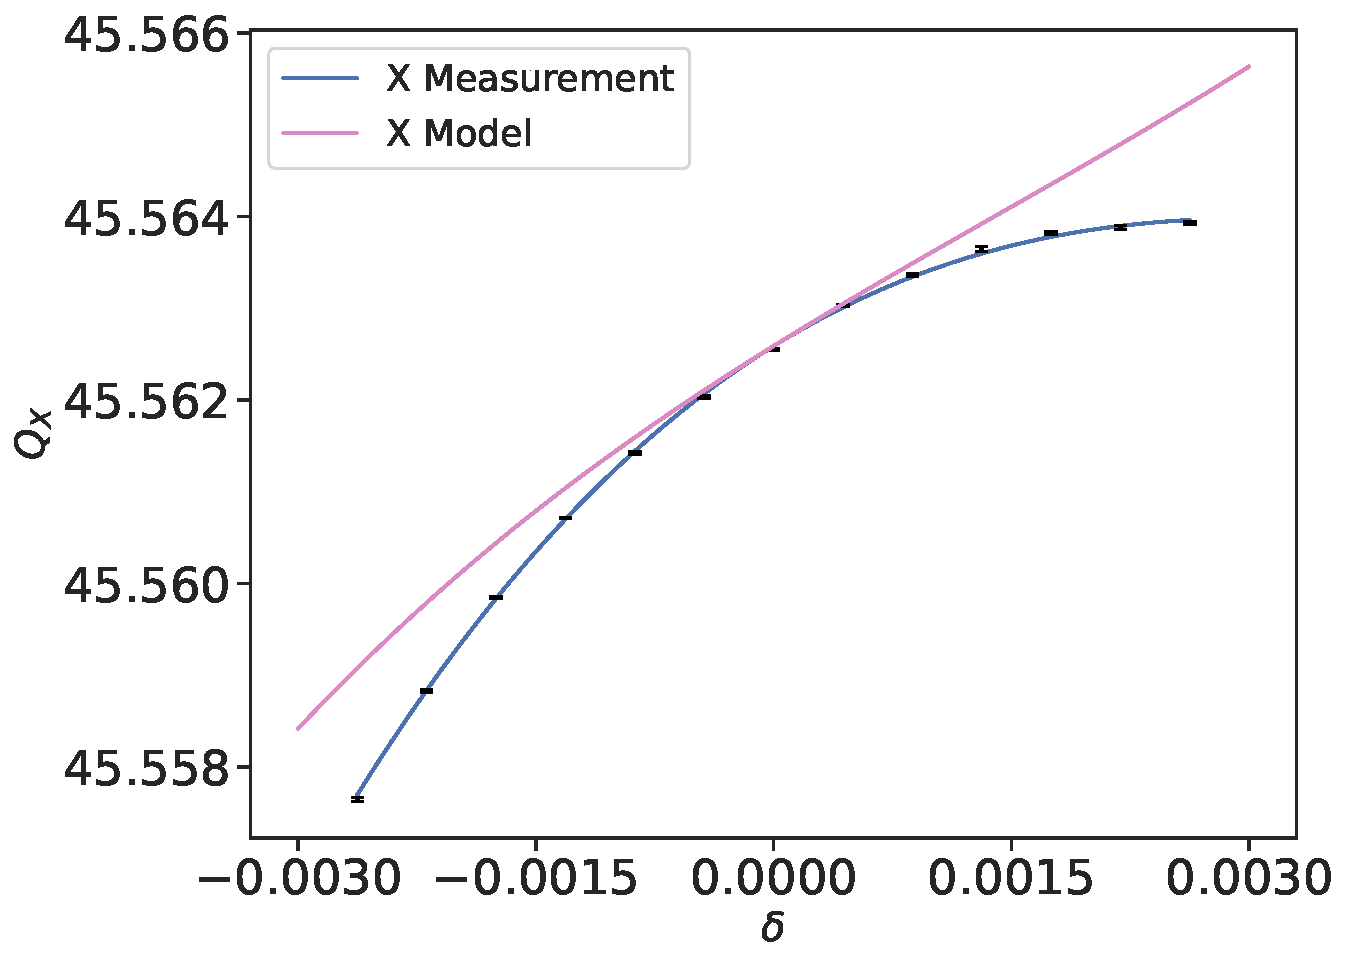
\includegraphics[width=\linewidth]{images/kek/chromaticity/HER_09/qx_modelq0q1.pdf}
        \caption{}
    \end{subfigure}
    \begin{subfigure}[b]{0.49\textwidth}
        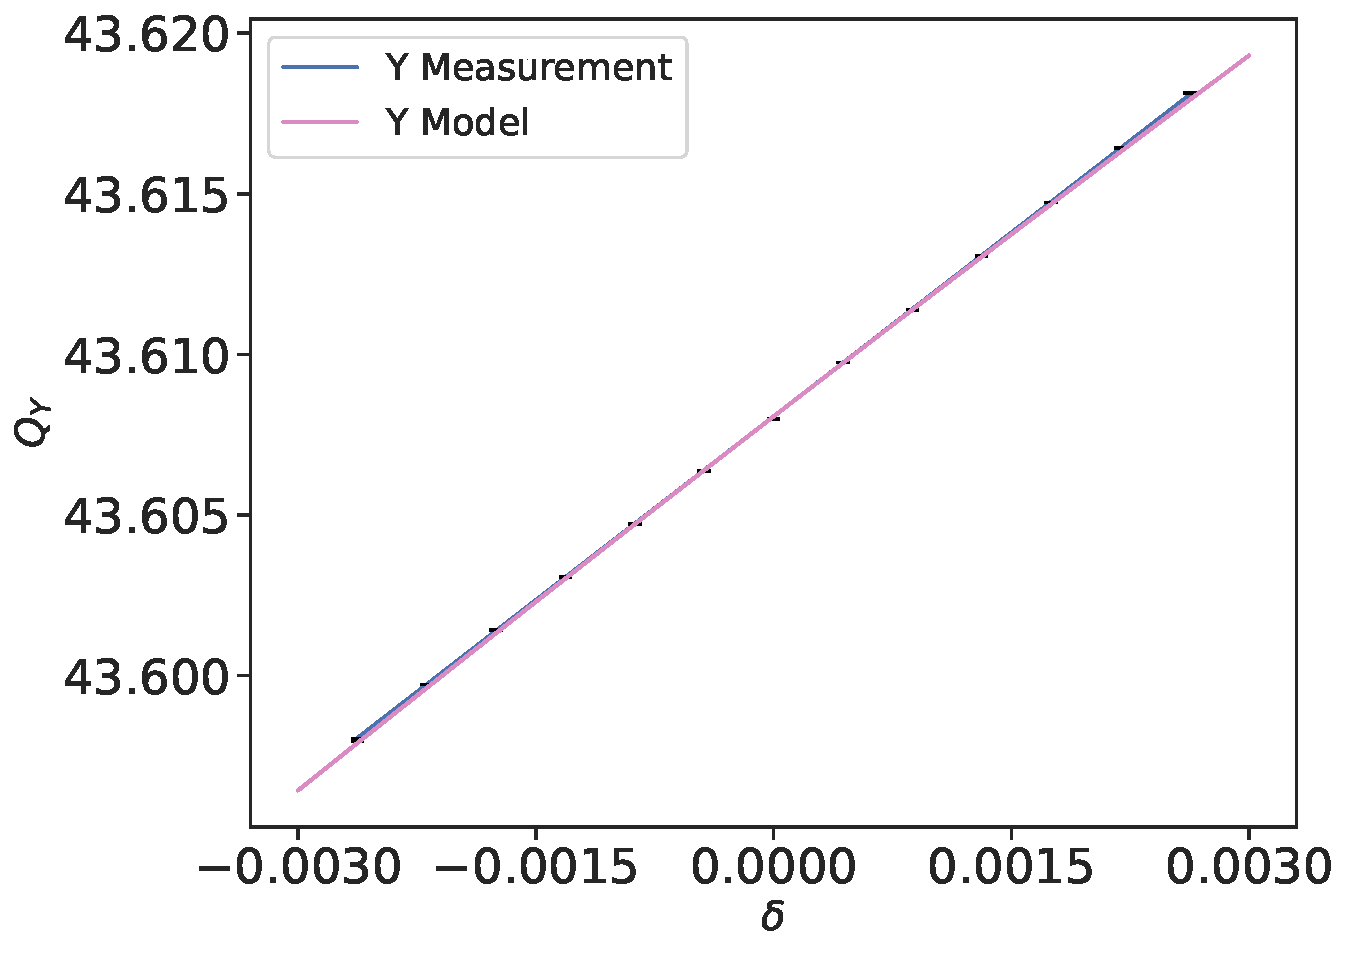
\includegraphics[width=\linewidth]{images/kek/chromaticity/HER_09/qy_modelq0q1.pdf}
        \caption{}
    \end{subfigure}
    \caption{}
    \label{fig:kek:chroma_HER_detuned}
\end{figure}

\begin{figure}[!htb]
    \centering
    \begin{subfigure}[b]{0.49\textwidth}
        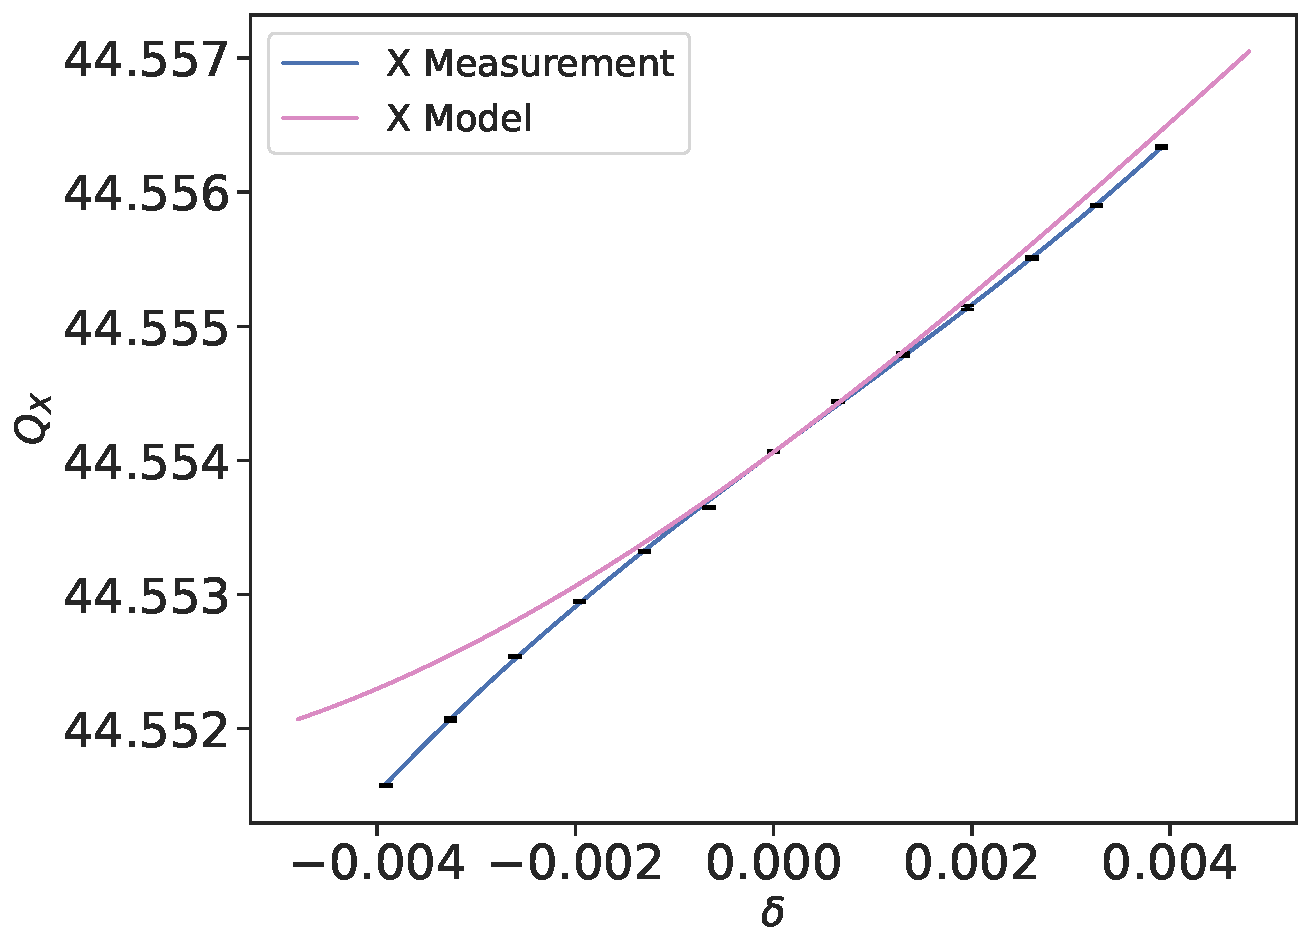
\includegraphics[width=\linewidth]{images/kek/chromaticity/LER_09/qx_modelq0q1.pdf}
        \caption{}
    \end{subfigure}
    \begin{subfigure}[b]{0.49\textwidth}
        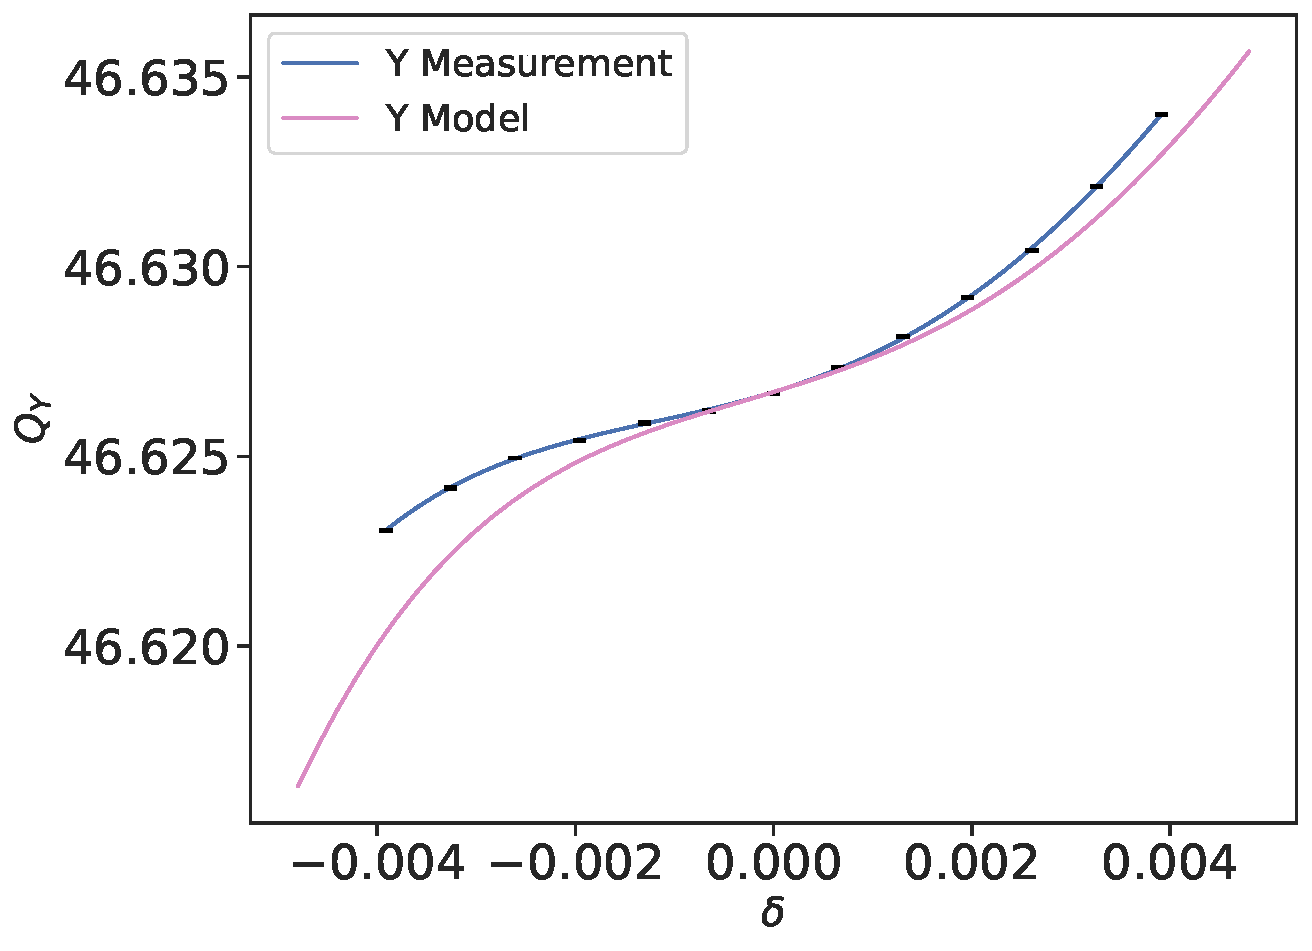
\includegraphics[width=\linewidth]{images/kek/chromaticity/LER_09/qy_modelq0q1.pdf}
        \caption{}
    \end{subfigure}
    \caption{}
    \label{fig:kek:chroma_LER_detuned}
\end{figure}


% HER detuned
\begin{figure}
    \centering
    \begin{minipage}[b]{0.49\textwidth}
        \centering
        \begin{table}
          \footnotesize
          \begin{tabular}{lrr}
            & $Q'' [\times 10^3]$ & $Q''' [\times 10^6]$ \\
            \midrule
            Meas.       &  -0.51 ± 0.01 & 0.11 ± 0.02\\
            Model       &  -0.12 ± 0.00 & 0.09 ± 0.00\\
            \bottomrule
          \end{tabular}
        \end{table}
    \end{minipage}
    \hfill
    \begin{minipage}[b]{0.49\textwidth}
        \centering
        \begin{table}
          \footnotesize
          \begin{tabular}{lr}
          & $Q'' [\times 10^3]$ \\
          \midrule
          Meas.       &  0.00 ± 0.0 \\
          Model       & -0.04 ± 0.0 \\
          \bottomrule
          \end{tabular}
        \end{table}
    \end{minipage}
\end{figure}

% LER detuned
\begin{figure}
    \centering
    \begin{minipage}[b]{0.49\textwidth}
        \centering
        \begin{table}
          \begin{tabular}{lrr}
            & $Q'' [\times 10^3]$ & $Q''' [\times 10^6]$ \\
            \midrule
              Meas. & -0.01 ± 0.0 &  0.02 ± 0.0 \\
              Model &  0.04 ± 0.0 & -0.01 ± 0.0 \\
            \bottomrule
            \end{tabular}
        \end{table}
    \end{minipage}
    \hfill
    \begin{minipage}[b]{0.49\textwidth}
        \centering
        \begin{table}
          \begin{tabular}{rrr}
            $Q'' [\times 10^3]$ & $Q''' [\times 10^6]$ & $Q^{(4)} [\times 10^9]$ \\
            \midrule
             0.35 ± 0.01 & 0.24 ± 0.01 & -0.09 ± 0.01 \\
             0.10 ± 0.00 & 0.32 ± 0.00 & -0.09 ± 0.00 \\
            \bottomrule
            \end{tabular}
        \end{table}
    \end{minipage}
\end{figure}


%=============================
%        Conclusion
%=============================
\FloatBarrier
\section{\todo{Summary}}

The measurements demonstrate excellent reproducibility of linear optics, with particularly improved
results in the horizontal plane when using a kicker. This reproducibility has been observed
consistently across several days and from shot to shot. Sextupolar Resonance Driving Term (RDT)
measurements in both rings have been conducted, although clean measurements could not always be
achieved, and some discrepancies remain to be clarified. Chromaticity measurements for both rings
were generally good; however, discrepancies in \( Q'' \) have been attributed to octupolar-like
sources, while LER’s \( Q''_y \) discrepancies are linked to decapolar-like sources. Additionally,
amplitude detuning for LER was measured with detuned optics, and a model comparison is expected to
provide a more detailed understanding of \( Q'' \).